\documentclass[12pt,oneside]{article}
\usepackage[utf8x]{inputenc}
\usepackage{mathtools}
\usepackage{titlesec}
\usepackage{indentfirst}
\usepackage{graphicx}
\usepackage{float}
\usepackage{amsmath}
\usepackage{url}
\usepackage{scrextend}
\usepackage{listings}
\usepackage[export]{adjustbox}
\usepackage[paper=a4paper]{geometry}
\usepackage{fontspec}
\setmainfont[Ligatures=TeX]{Calibri}
\renewcommand{\contentsname}{Cuprins}
\renewcommand{\refname}{Bibliografie}
%\usepackage{fontspec}
%\setmainfont[Ligatures=TeX]{UTSans}
%\usepackage[paper=a4paper,left=2cm,right=2cm,top=2cm,bottom=2cm]{geometry}

\usepackage{fancyhdr}
\pagestyle{fancy}
\fancyhf{}
\cfoot{\thepage}
\rfoot{
\includegraphics[scale=0.15]{sigla_footer.png}}
\renewcommand{\headrulewidth}{0pt}

\fancypagestyle{plain}{%
	\fancyhf{} 
	\rfoot{
\includegraphics[scale=0.15]{sigla_footer}}
	\cfoot{\thepage}
	\renewcommand{\headrulewidth}{0pt}% Line at the header invisible
}

\fancypagestyle{empty}{%
	\fancyhf{} 
	\rfoot{
\includegraphics[scale=0.15]{sigla_footer.png}}
	\renewcommand{\headrulewidth}{0pt}% Line at the header invisible
}

\graphicspath{{images/}}
\everymath{\displaystyle}
\setlength{\parskip}{1em}
\setcounter{secnumdepth}{4}

\title{Separarea surselor}
\author{Motrescu Radu}
\date{}

\begin{document}
\thispagestyle{empty}
\begin{titlepage}
	%\newgeometry{top=1in,bottom=1in,right=0.5in,left=1.5in}
	\begin{center}
\begin{figure}[H]
			\begin{minipage}[l]{70pt}
				
\includegraphics[scale=0.4]{sigla}
			\end{minipage}
			\begin{minipage}[c]{300pt}
				\begin{flushright}
					{\large}{Programul de studii:\\	\vspace{0.3em}
							Informatică}
				\end{flushright}
			\end{minipage}
		\end{figure}
        \centering
        \vspace{4\baselineskip}
        {\Huge
        \textbf{Lucrare de licență}\\ \textbf{Separarea surselor independente}\par}
        \vspace{15\baselineskip}
		\par
		\begin{flushleft}
        {\large{Autor: \hspace{33mm}	\textbf{Radu-Marian Motrescu}}\par}
        {\large{Coordonator științific: \hspace{1mm} \textbf{Lect. Dr. Honorius-Cezar Gâlmeanu}}\par}
		\end{flushleft}
		\vfill
		\par
        %\vspace{16\baselineskip}
        {\Large{Brașov, 2018}\par}
    \end{center}
\end{titlepage}

\pagestyle{plain}

\newpage
\setcounter{page}{1}
\tableofcontents
\clearpage

\newpage

\pagestyle{plain}
\section{Introducere in analiza si separarea componentelor}
Aceasta lucrare are scopul de a informa cititorul asupra unor metoda de analizare a componentelor unor date, fie acestea date economice sau imagini, pentru a putea fi interpretate mai usor, cat si metode de separare a componentelor unui set de date. 

Algoritmii abordati sunt \textbf{PCA (Principal Component Analysis)}, \textbf{KPCA (Kernel Principal Component Analysis)} si \textbf{ICA (Independent Component Analysis)}. 

O scurta descriere a cazurilor de aplicare a algoritmilor mentionati:
\begin{itemize}
	\item{PCA - Este folosit pentru a extrage informatiile cele mai relevante dintr-un set de date, adeseori cu dimensionalitate mare, cu scopul atat de a face interpretarea lor mai usoara, cat si pentru prelucrarea lor mai rapida, prin proiectarea a noi feature-uri ale setului de date obtinute prin combinari liniare ale celor existente, obtinand astfel directiile de maxima variabilitate.}
	\item{KPCA - Este o extensie a PCA, si acopera slabiciunile PCA, spre exemplu in seturi de date in care distributia valorilor nu poate fi analizata la fel de bine de PCA, si in cazuri de clustering, feature-urile noi ale setului de date se obtin prin combinari neliniare ale celor vechi.}
	\item{ICA - Aceasta abordare de analizare a componentelor are avantajul de le putea si separa din punct de vedere statistic, si este adeseori folosita in cazuri de separare a semnalelor de diferite tipuri, precum audio si video.}
\end{itemize}

\newpage

\section{PCA}

\subsection{Ce este PCA?}
PCA, sau Principal Component Analysis, sau pe romaneste, Analiza Componentelor Principale este o unealta matematica aplicata din algebra liniara. Este o metoda non-parametrica (care nu depinde de statistici) de a extrage informatiile relevante dintr-un set de date complex sau confuz.\cite{data_reduction}

\paragraph{Un scurt exemplu: \cite{data_reduction}}
Sa presupunem ca am extras informatii pentru 100 de parametri pentru un student: inaltime, varsta, greutate, nota obtinuta la un test, culoarea parului etc. Vrem sa gasim cele mai importante caracteristici care definesc studentul. Cum facem asta? Folosim PCA pentru a le selecta.

\begin{itemize}
	\item Ce parametri dorim sa ignoram mergand mai departe cu setul de date:
	\begin{itemize}
	\item Constanti: numarul de capete, care este 1 pentru toti studentii
	\item Aproape constanti: grosimea firului de par: 0.003, 0.002, 0.0005 etc.
	\item Care depind de alti parametri
	\end{itemize}
	\item Ce parametri dorim sa pastram:
	\begin{itemize}
	\item Care nu depind de alti parametri: culoarea ochilor
	\item Care se schimba mult, au variatie mare: notele
	\end{itemize}
\end{itemize}

A putea elimina parametrii irelevanti si a-i pastra pe cei relevanti este usor pentru un om, el putand vedea clar care parametri nu exprima informatii relevante despre subiectul respectiv, dar cum putem face calculatorul sa isi dea seama de acesti parametri? Folosind matematica, desigur!

Dorim sa minimizam "sunetul de fundal" si redundanta datelor si sa maximizam variatia dintre parametri.

Se poate vedea in imaginea de mai jos maximizarea variatiei dintre axele norului de puncte respectiv.\cite{pca_shlens}

\begin{figure}[H]
\centering
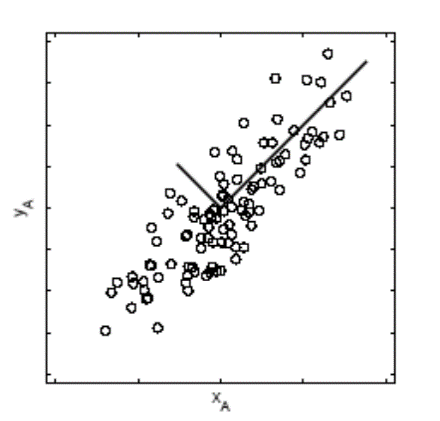
\includegraphics[scale=0.5]{Picture1}
\end{figure}

In imaginile de mai jos se pot vedea inregistrarile unor informatii. In imaginea (a) si (b) se poate vedea cum informatiile nu sunt corelate, avand redunanta mica spre medie (ex: inaltimea unui student si media lui), iar in imaginea (c) se poate vedea o redundanta mare, insemnand ca ambii parametrii pot fi exprimati unul in functie de celalalt.\cite{pca_shlens}

\begin{figure}[H]
\centering
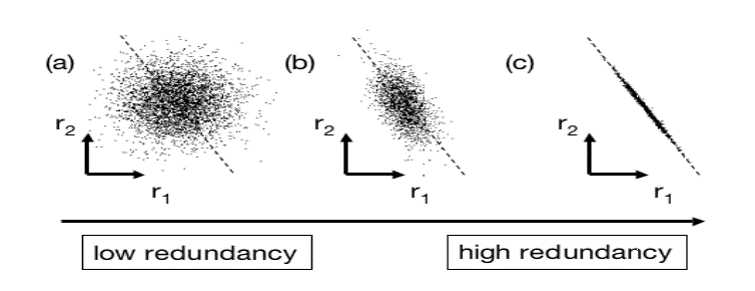
\includegraphics[width=\linewidth]{Picture2}
\end{figure}

\paragraph{Deviatia standard} Este un mijloc de realizare a variabilitatii datelor dintr-un set de date cu media $\overline{X}$:

\begin{equation}
\sigma^2=\frac{\sum_{i=1}^{n} \left( X_i - \overline{X} \right)^2 }{n-1}
\end{equation}


\paragraph{Covariatia} Reprezinta variabilitatea fiecarei dimensiuni in relatie cu celelalte, si este masurata intre 2 dimensiuni pentru a se putea observa relatia dintre cele 2, spre exemplu numarul de ore studiate si nota obtinuta la examen.

\begin{equation}
\text {var} \left( X \right) = \frac{\sum_{i=1}^{n} \left( X_i - \overline{X} \right) \left( X_i - \overline{X} \right) }{n-1}
\end{equation}


\begin{equation}
\text {cov} \left( X,Y \right) = \frac{\sum_{i=1}^{n} \left( X_i - \overline{X} \right) \left( Y_i - \overline{Y} \right) }{n-1}
\end{equation}

Pe langa aceste masuratori exista si coeficientul de corelatie Pearsson:

\begin{equation}
	p(x,y)=\frac{\text{cov}(X,Y)}{\sigma x \sigma y}
\end{equation}

Aceasta masura a corelatiei liniare dintre doua variabile aleatoare $X$ si $Y$ poate lua valori intre $-1$ si $+1$, unde $+1$ este o corelatie totala pozitiva, $0$ inseamna nici o corelatie liniara, iar $-1$ este corelatie totala negativa.\cite{pearsson_correlation_coefficient_wiki}

\paragraph{Matricea de covariatie}
Consideram setul de date din care extragem valoarea medie, rezultand date centrate (zero-mean data) si avand setul de vectori \( \left\{ x_1, x_2, ..., x_m \right\} \) care reprezinta liniile unei matrici $X_{m,n}$.

Fiecare linie a matricii reprezinta toate masuratorile unui anumit parametru, iar fiecare coloana reprezinta masuratorile care s-au intamplat la un moment dat.

De aici ajungem la definitia matricei de covariatie:

\begin{equation}
S_x \equiv \frac{1}{n-1}XX^T \text { where } X = 
\begin{bmatrix}
x_1 \\ \vdots \\ x_m
\end{bmatrix}
\end{equation}

$S_x$ este o matrice simetrica $m \times m$, termenii de pe diagonala reprezentand variatia din acelasi parametru, iar termenii care nu sunt de pe diagonala reprezinta covariatia dintre parametri diferiti. Calculand $S_x$, cuantificam corelatia dintre toate posibilele perechi de masuratori. Observand elementele din matrice, o covariatie mare reprezinta un caz de redundanta mare, iar o covariatie egala cu 0 reprezinta date complet necorelate.

\begin{equation}
C=\begin{bmatrix}
cov(X,X) && cov(X,Y) && cov(X,Z) \\
cov(Y,X) && cov(Y,Y) && cov(Y,Z) \\
cov(Z,X) && cov(Z,Y) && cov(Z,Z)
\end{bmatrix}
\end{equation}


\paragraph{Valorile si vectorii proprii}
Urmatorul pas in calcularea PCA este aflarea valorilor si a vectorilor proprii ale matricii de covariatie. Extragand aceste informatii, ele ne vor arata componentele principale ale setului de date: vectorul propriu cu cea mai mare valoare proprie este componenta principala a setului de date. Se obisnuieste sortarea vectorilor proprii in functie de valoarea proprie pentru a determina ordinea de semnificativitate.

Vectorii si valorile proprii reies din probleme de urmatoarea forma:
\begin{equation}
A.v= \lambda . v
\end{equation}

\textbf{$A$}: matrice $m \times m$


\textbf{$v$}: vector $m \times 1$  nenul


$\lambda$: constanta

Pentru orice valoare a lui $\lambda$ pentru care ecuatia are solutie se numeste valoarea proprie a lui $A$, si vectorul $v$ care corespunde acestei valori se numeste vectorul propriu a lui $A$. 

Pentru fiecare vector se calculeaza contributia lui la deviatia standard totala, data de valoarea proprie asociata lui:

\begin{equation}
	\text{contrib}(a)=\frac{a}{\sum_{i=0} A_i}
\end{equation}

Contributiile vectorilor proprii care corespund valorilor proprii celor mai mari vor avea un procentaj al deviatiei standard ridicat, si astfel in general se ajunge la cazul in care primele trei sau patru componente ocupa de la $80\%$ pana la $95\%$ din procentajul de deviatie standard total. Urmarind aceste procentaje putem decide ce componente vor fi alese pentru a ramane in setul de date pentru a fi procesate in continuare.


\paragraph{Pasul final PCA} este sa aflam valorile finale ale setului de date. Dupa stabilirea vectorilor proprii doriti, aflarea datelor finale este simpla, proiectam punctele in spatiul lor: 

FinalData = RowFeatureVector $\times$ RowZeroMeanData

\textbf{RowFeatureVector} este matricea cu vectorii proprii transpusi, cu cel mai semnificati vector propriu pe prima linie.

\textbf{RowZeroMeanData} este matricea care contine setul de date initial din care s-a scazut valorea medie.

Matricea rezultata \textbf{FinalData} va contine setul de date dupa aplicarea algoritmului PCA.

\subsection{Biblioteca Accord.NET}
Biblioteca Accord.NET este o biblioteca pentru limbajul C\#, fiind disponibila prin pachetele NuGet si contine clase pentru:
\begin{itemize}
\item Calcul stiintific: matematica, statistica si machine learning
\item Procesare de imagini si semnale: imagini, semnale audio si recunoastere si urmarire faciala in timp real
\item Biblioteci suport pentru controale specifice: histograme, scatter-plots, controale pentru fiecare clasa de procesare imagini si semnale
\end{itemize}

In contextul cerintelor pe care vrem noi sa le indeplinim, vom folosi clase dedicate matematicii, statisticii, si ale unor controale de afisare a datelor.

Implementarea aplicatiilor corespunzatoare algoritmilor PCA s-a facut in mediul de programare Visual Studio, cu limbajul de programare C\#.

\subsection{Aplicatia AccordPCA}
Primii pasi pe care i-am facut in cadrul acestui proiect a fost implementarea algoritmului PCA. Acest lucru a fost realizat usor, folosind libraria Accord, mai specific, pentru a realiza diferitele operatii cu matrici. \cite{accord_pca}

\begin{lstlisting}[basicstyle=\footnotesize]
public void Compute()
{
	mean = initialData.Mean(0);

	dataAdjusted = initialData.Subtract(mean, 0);
	covarianceMatrix = dataAdjusted.Covariance();

	evd = new EigenvalueDecomposition(covarianceMatrix);

	eigenvalues = evd.RealEigenvalues;
	eigenvectors = evd.Eigenvectors;

	eigenvectors = Matrix.Sort(eigenvalues, eigenvectors,
			new GeneralComparer(ComparerDirection.Descending, true));

	finalData = dataAdjusted.Dot(eigenvectors);

	data2D = finalData.GetColumns(0, 1);
}
\end{lstlisting}
%\begin{figure}[H]
%\centering
%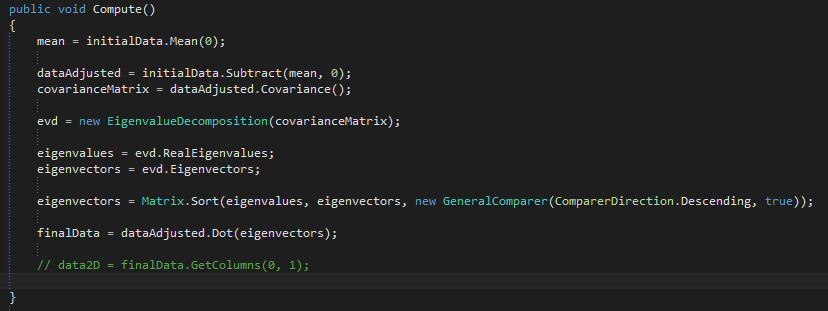
\includegraphics[width=\linewidth]{Compute}
%\end{figure}

Pentru a testa acest algoritm, am introdus prima data un set de date deja testat, unde se poate observa clar rezultatul algoritmului.\cite{data_reduction}
\begin{figure}[H]
\centering
\caption{Primul test PCA}
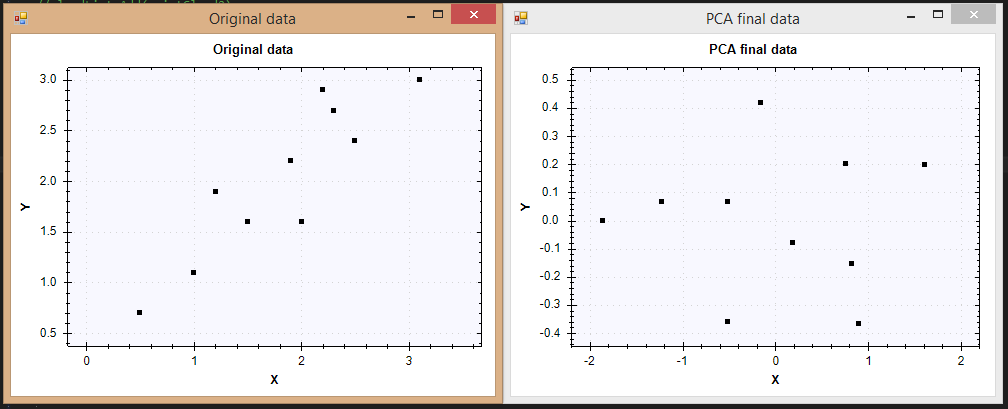
\includegraphics[width=\linewidth]{Test1}
\end{figure}
\newpage

Urmatorul lucru pe care l-am dorit sa il facem a fost sa vedem cum mai multi nori de puncte, de diferite dimensiuni, se modifica dupa aplicarea algoritmului. Pentru acest lucru, am creat o clasa \textbf{PointCloud} care descrie un nor de puncte. In interiorul clasei am generat norul de puncte in jurul unor coordonate $\left(x,y\right)$, sub forma unui disc, in care punctele au distributie normala. Rezultatele au fost urmatoarele:

\begin{figure}[H]
\centering
\caption{Al doilea test PCA}
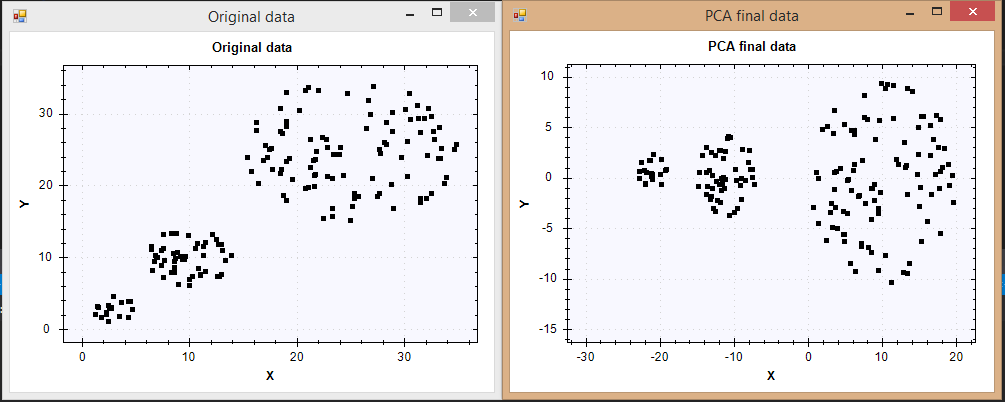
\includegraphics[width=\linewidth]{Test2}
\end{figure}

La fel ca in primul test, se poate observa aranjarea dupa prima componenta principala a norilor. Cand vorbim de aceasta aranjare, vorbim defapt de miscari in plan, si sunt reprezentate prin inmultiri ale setului de date cu matrici care corespund translatiei si rotatiei, lucru care se intampla si in cazul nostru, matricea de translatie si rotatie fiind matricea vectorilor proprii.

Aceasta aplicatie a fost folosita mai departe pentru a implementa ceilalti algoritmi PCA folositi, elementele de UI fiind eliminate.

\newpage
\subsection{Aplicatia PlotPCA}
In acest moment, am decis sa realizam o aplicatie care are un GUI usor de folosit si unde fiecare nor de puncte este reprezentat in alta culoare, pentru a se vedea mai clar ce se intampla, acest lucru fiind mai important pentru seturile de date in care masuratorile pentru fiecare entitate sunt intrepatrunse.

\subsubsection{Setul 3-cloud-points}
Primele teste pe care le-am facut, au fost pe trei nori de puncte generati aleator, la fel ca in exemplul de mai sus, si se poate vedea mai clar separarea norilor atat in spatiul 2D, cat si pe axa primei componente, cea cu variatie maxima. \begin{figure}[H]
	\caption{Nori separati total}
	\centering
	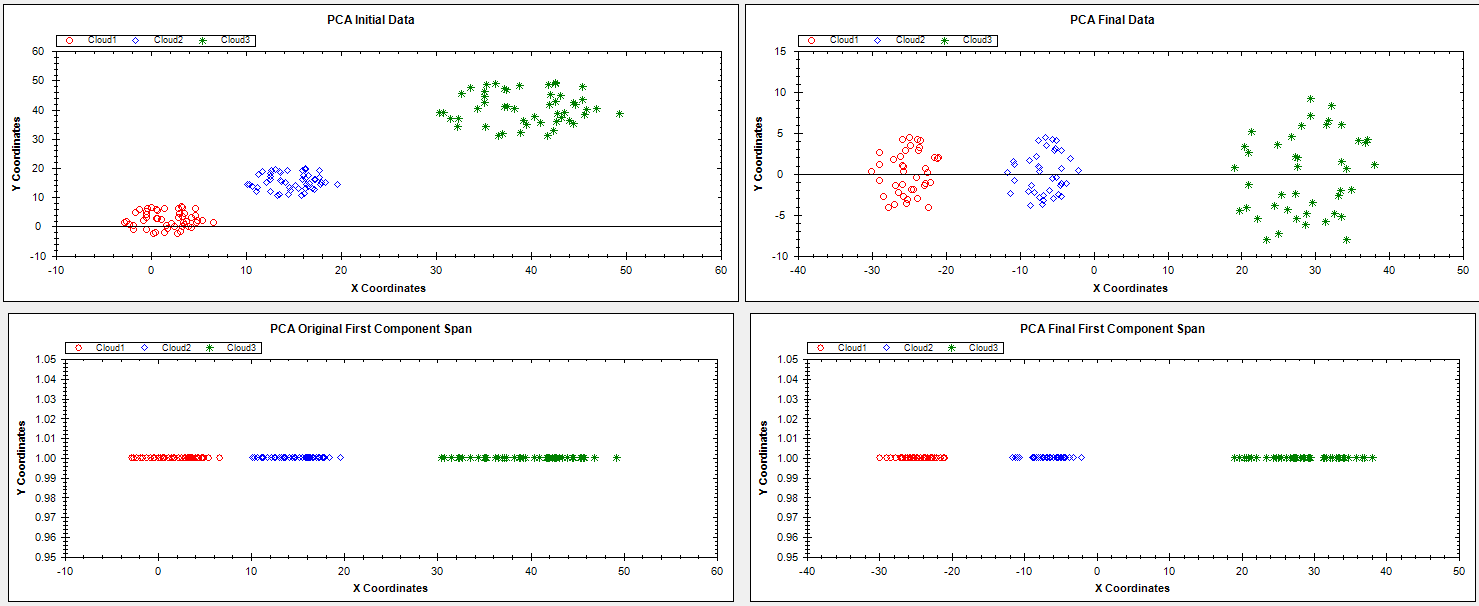
\includegraphics[width=\linewidth]{threecloud1}
\end{figure}

De asemenea, atunci cand norii se suprapun putin de-a lungul axei Y, algoritmul PCA reuseste sa separe norii complet de-a lungul axei primei componente. 

\begin{figure}[H]
\caption{Nori intersectati partial}
\centering
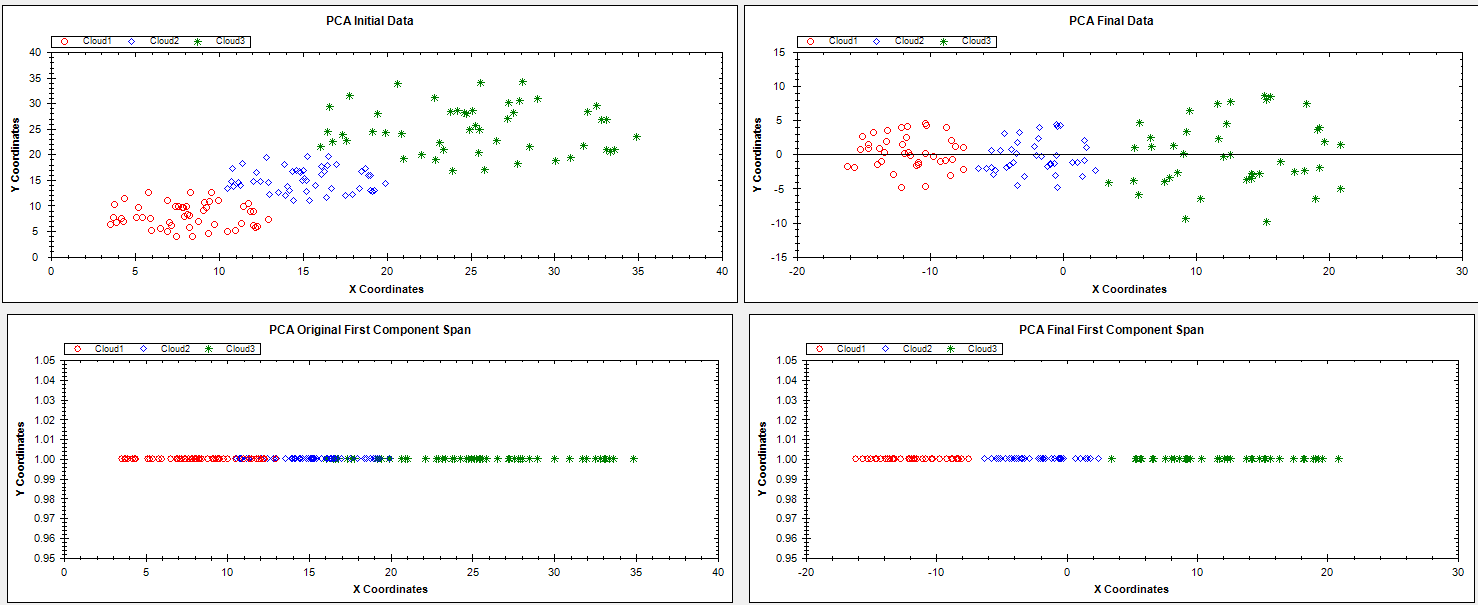
\includegraphics[width=\linewidth]{threecloud2}
\end{figure}

Pe de alta parte, daca norii se suprapun mai mult, atunci se poate observa ca algoritmul PCA nu ii mai poate separa la fel de bine.

\begin{figure}[H]
\centering
\caption{Norul albastru si verde intersectati aproape total}
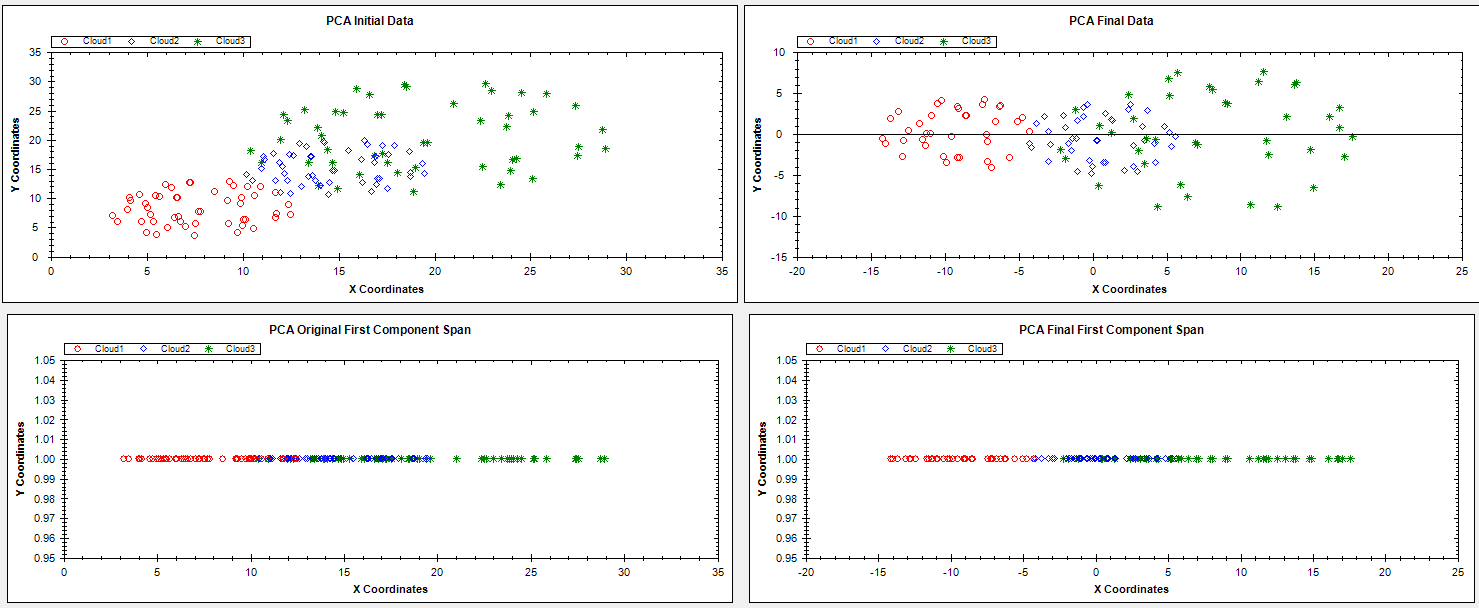
\includegraphics[width=\linewidth]{threecloud3}
\end{figure}

\newpage
\section{Kernel PCA}

\subsection{Setul two-moon si abordarea Kernel PCA}
Pentru a aborda problema seturilor de date liniar inseparabile, nu putem folosi abordarea PCA simpla, rezultatul nu va fi cel dorit, dupa cum se poate vedea aplicand algoritmul PCA pentru setul two-moon: cele doua seturi de puncte se amesteca de-a lungul primei componente principale, astfel o clasificare a unui nou punct proiectat in spatiul respectiv va fi dificila, deoarece nu putem seta un punct de delimitare intre cei doi nori, acestia fiind intrepatrunsi. 

Abordarea Kernel PCA rezolva acest lucru prin proiectarea feature-urilor setului de date din spatiul defectuos neliniar, intr-un spatiu dimensional mai mare, dat de vectorii proprii, unde ele vor deveni liniar separabile, iar acest lucru se face cu o "functie kernel". Vom prezenta aceasta abordare conform articolului lui Sebastian Raschka.\cite{kernel_pca}

Pentru a implementa Kernel PCA, vom avea in considerare urmatoarele 2 lucruri:

\textbf{1. Calcularea matricii kernel} 

Pentru fiecare pereche de puncte se calculeaza :

\begin{equation}
k(x_i,x_j)=\exp(-\gamma \|x_i - x_j\|_2^2)
\end{equation}

Daca avem un set de date cu 100 de mostre, matricea kernel va fi o matrice simetrica $100 \times 100$.

Alegerea valorii lui $\gamma$ este foarte importanta, in functie de ea rezultatul va fi cel dorit sau nu.

\textbf{2. Calcularea vectorilor si a valorilor proprii}

Deoarece nu putem garanta ca matricea e centrata, vom aplica urmatoarea formula pentru a o centra: 

\begin{equation}
K'=K-1_NK-K1_N+1_NK1_N
\end{equation}

unde $1_N$ este o matrice $N \times N$ cu toate valorile egale cu $\frac{1}{N}$.
Acum, putem afla vectorii si valorile proprii pentru matricea centrata, iar vectorii proprii vor reprezenta setul de date proiectat pe componentele principale respective.

In imaginile urmatoare se poate observa cum algoritmul PCA si algoritmul KPCA afecteaza setul de date two-moon, rezultatul obtinut prin folosirea KPCA este mult mai bun. 


\begin{figure}[H]
\centering
\caption{Setul two-moon proiectat cu ajutorul algoritmul KPCA, $\gamma =15$}
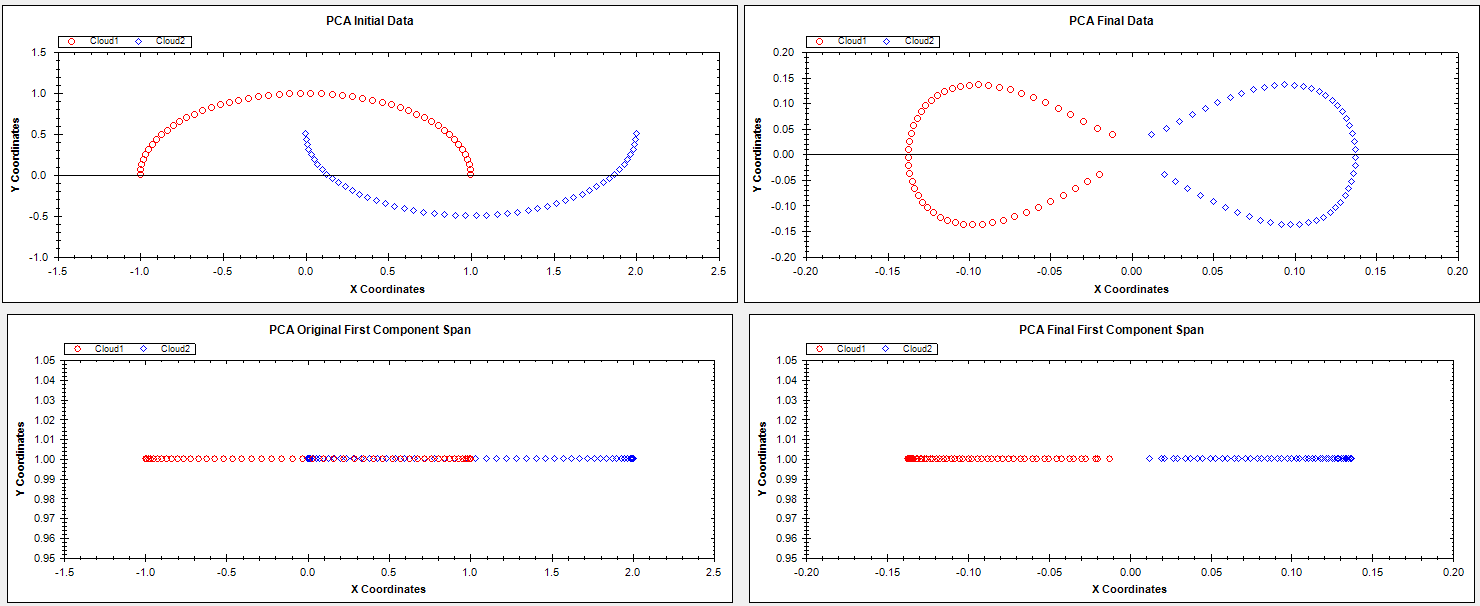
\includegraphics[width=\linewidth]{twomoon1}
\end{figure}

\subsection{Cros-validare 10-fold}
Pentru a ne asigura ca algoritmul se comporta corect si in alte situatii, am decis sa facem o cros-validare 10-fold (10-fold cross-validation). Acest lucru implica urmatoarele: 

-avem 100 de puncte, distribuite in setul de date two-moon

-din acestea, vom alege pe rand, cate 10 puncte, diferite de fiecare data, si vom retine norul din care face parte fiecare

-cu celelalte 90 de puncte vom antrena algoritmul pentru a putea proiecta celelalte 10 puncte pe componentele principale respective, in cazul nostru, dorim sa facem proiectarea pe prima componenta principala

-avand cele 90 de puncte proiectate in spatiul nou, putem determina din nou granitele celor 2 nori de puncte, iar mijlocul acestor granite va fi punctul nostru de separare a norilor

-cu punctul de separare gasit, cele 10 puncte proiectate pe prima componenta principala pot fi categorizate: daca se afla in stanga punctului de separare el va fi in norul albastru de puncte, iar daca este la dreapta punctul de separare, va apartine norului rosu

-stiind din ce nori au provenit punctele si in ce nori au fost proiectati, putem verifica eroarea algoritmului pentru cele 10 puncte: $\frac{nr. \text { } puncte \text { } proiectate \text { } gresit}{nr. \text { } puncte \text { } totale}$

-repetam acest proces pana cand toate punctele au fost proiectate, iar eroarea de final este cea cautata

In cazul testelor noastre, eroarea a variat intre 1\% si 4\%, fiind un rezultat foarte bun.

\begin{figure}[H]
\centering
\caption{Exemplu de validare 10-fold}
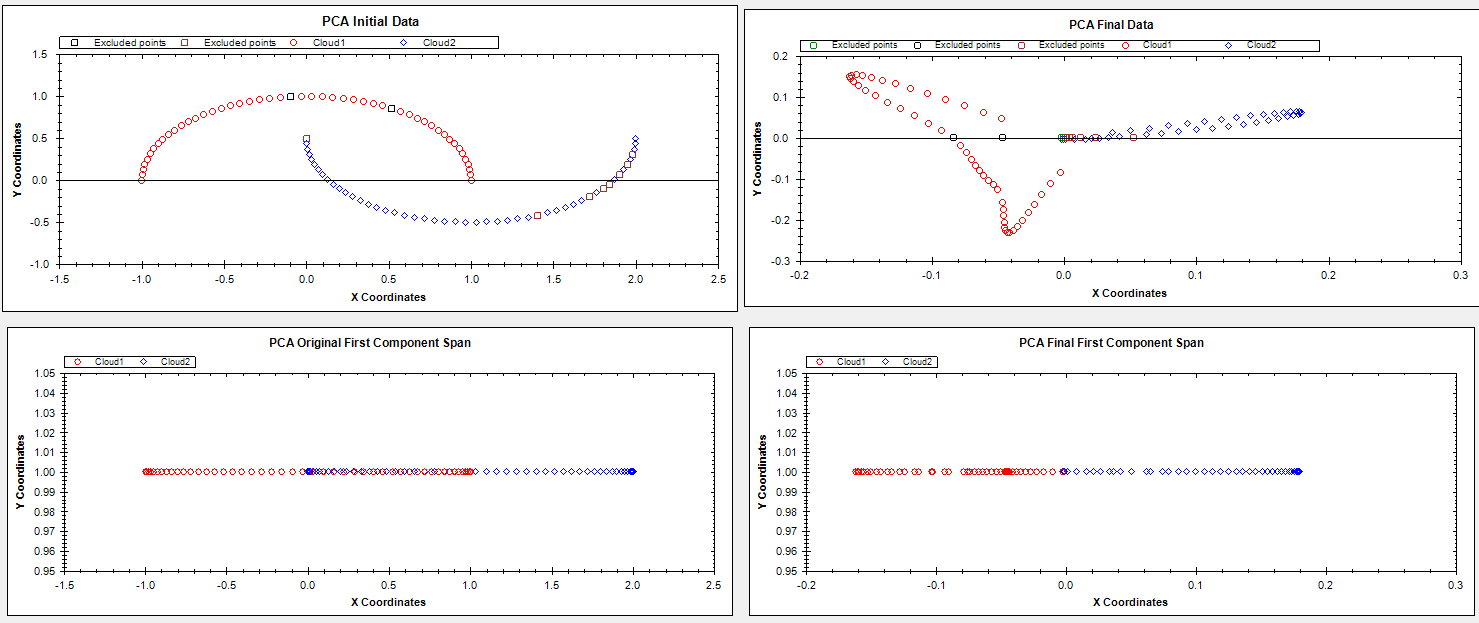
\includegraphics[width=\linewidth]{tenfold1}
\end{figure}

\newpage

\subsection{Aplicatia Eigenfaces}
Dupa ce am realizat testele KPCA, urmatorul pas a fost sa crestem dimensiunile cu care lucram. Mai exact, am inceput sa folosim imagini pentru a vedea cum actioneaza algoritmul PCA pe ele.

Imaginile folosite au fost cele din baza de date Yale, care a fost folosita in multe alte cercetari de genul acesta, continand destui subiecti si destule imagini pentru a putea testa orice algoritm.\cite{yale_db} \cite{KCLee05}

Pentru a putea procesa aceste imagini, ele trebuiau sa aiba toate aceeasi dimensiune, in cazul nostru $168 \times 192$, iar fiecare imagine va deveni un rand din matricea care va fi prelucrata de algoritmul PCA.

Fetele rezultate din acest algoritm reprezinta toti vectorii proprii care contribuie la spatiul fetelor intr-un mod semnificativ, si sunt sortati dupa valoarea proprie, si dupa cum se poate observa, aceste imagini devin din ce in ce mai nesemnificative: 

\begin{figure}[H]
\centering
\caption{Primele 10 eigenfaces-uri ale celui de-al treilea subiect}
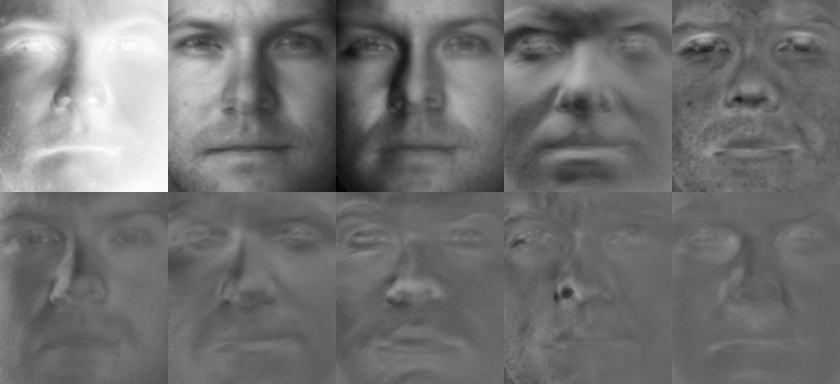
\includegraphics[width=\linewidth]{eigenfaces}
\end{figure}

\subsubsection{Proiectarea unei imagini noi}
Pentru a putea proiecta o imagine noua in spatiul fetelor, tot ce trebuie sa facem este: 

\begin{equation}
X=X-avg(X)
\end{equation}
\begin{equation}
Y=X^T \times E_0
\end{equation}

$X=$ este vectorul imaginii pe care o vom proiecta

$E_0=$ este vectorul propriu asociat valorii proprii maxime

$Y=$ este imaginea proiectata.

\subsubsection{Clasificarea unei imagini noi}

Pentru a vedea daca o imagine nou proiectata apartine sau nu setului initial de imagini, avem nevoie mai intai de imaginea proiectata, si de o granita, la fel ca la abordarea KPCA.

Modul prin care vom afla daca o imagine apartine setului este prin calcularea distantei de la aceasta imagine la reprezentarea setului de imagini in spatiul respectiv, iar daca valorea aceasta este mai mica decat granita mentionata mai sus, imaginea va fi clasificata ca va apartine setului initial.

Pentru a afla aceasta distanta, vom efectua urmatoarele operatii:

\begin{equation}
D=W_i-Y
\end{equation}
\begin{equation}
N=\| D_i  \|
\end{equation}
\begin{equation}
v=min(N)
\end{equation}

$W=$ reprezinta fetele setului de date initial proiectate in spatiul fetelor

$D=$ diferenta dintre toate liniile lui $W$ si $Y$

$N=$ norma fiecarei linii din $D$

$v=$ este distanta dintre imaginea nou proiectata si spatiul fetelor

Pentru a afla granita care delimiteaza imaginile din spatiul fetelor de celelalte, vom folosi aceleasi operatii ca si mai sus, dar aplicate pe toate imaginile setului initial, si vom cauta $v=avg(N)$, distanta medie dintre toate fetele proiectate si spatiul fetelor. Am ales sa facem acest lucru si sa nu cautam $v=max(N)$ deoarece se poate intampla ca o imagine din setul initial sa aiba distanta fata de spatiul fetelor disproportional mai mare fata de celelalte, si astfel granita de clasificare ar fi prea mare, incluzand orice imagine pe care incercam sa o proiectam.

Acestea fiind zise, am facut urmatorul test: din cele 65 de imagini ale subiectului 1 din baza de date Yale, primele 44 au fost folosite pentru a "antrena" algoritmul, iar ultimele 21 au fost folosite pentru clasificare. Eroarea rezultata a fost de $\sim$ 50\%, imaginile care nu au fost clasificate ca facand parte in set au fost cele in care subiectul are numai jumatate de fata iluminata, numarul acestor imagini fiind $\sim$ 50\% din ele, deci putem trage concluzia ca algoritmul face ceea ce isi propune. 

\newpage
\section{ICA}

\subsection{Ce este ICA? }
Una dintre problemele din lumea reala este gasirea unei reprezentari potrivite pentru date multivariate, adica date care au multe dimensiuni, si care de multe ori sunt aleatoare. Din cauza problemelor de performanta, orice fel de reprezentare este deobicei interpretata ca o transformare liniara a datelor originale. Printre aceste metode de analiza a transformarilor liniare se numara si PCA, despre care am vorbit pana acum. ICA (Independent Component Analysis) sau Analiza Componentelor Individuale este o abordare noua care are rolul de a reprezentarile liniare ale unor date cu distributie nongaussiana, astfel incat componentele sa fie cat mai independente din punct de vedere statistic. Acest tip de separare este dorita deoarece captureaza structura esentiala a datelor in multe tipuri de aplicatii, precum extragerea caracteristicilor (feature extraction) sau separarea semnalelor (signal separation). Aceasta introducere cat si partea teoretica ce urmeaza este prezentata conform articolului publicat de Aapo Hyvärinen si Erkki Oja.\cite{hyvarien}

Pentru a putea vizualiza aceasta idee, putem analiza o problema din lumea reala. Sa spunem ca suntem intr-o camera in care 2 oameni vorbesc simultan. Avem 2 microfoane pe care le pozitionam in locuri diferite in camera, si ele ne dau 2 inregistrari ale semnalelor. Aceste semnale sunt $x_1 (t)$ si $x_2 (t)$, cu $x_1$ si $x_2$ functii de amplitudine in functie de $t$. Fiecare inregistrare este o suma ponderata a semnalelor emise de cei doi oameni care vorbesc, pe care le notam $s_1(t)$ si $s_2(t)$. Pentru claritate le punem sub forma de ecuatie liniara:

\begin{equation}
	x_1(t)=a_{11} s_1 + a_{12} s_2
\end{equation}
\begin{equation}
	x_2(t)=a_{21} s_2 + a_{22} s_2
\end{equation}

unde $a_{11}, a{12}, a_{21}, a_{22}$ sunt niste parametrii care determina distanta dintre microfoane si vorbitori. Avand aceste date, daca am putea estima cele doua semnale initiale $s_1(t)$ si $s_2(t)$ folosind doar semnalele inregistrate $x_1(t)$ si $x_2(t)$, am reusi sa rezolvam multe probleme din lumea reala. Tipul de problema prezentat mai sus este denumit si \textbf{cocktail-party problem}.

In imaginea urmatoare avem o reprezentare vizuala a problemei \cite{noise_reduction}:

\begin{center}
	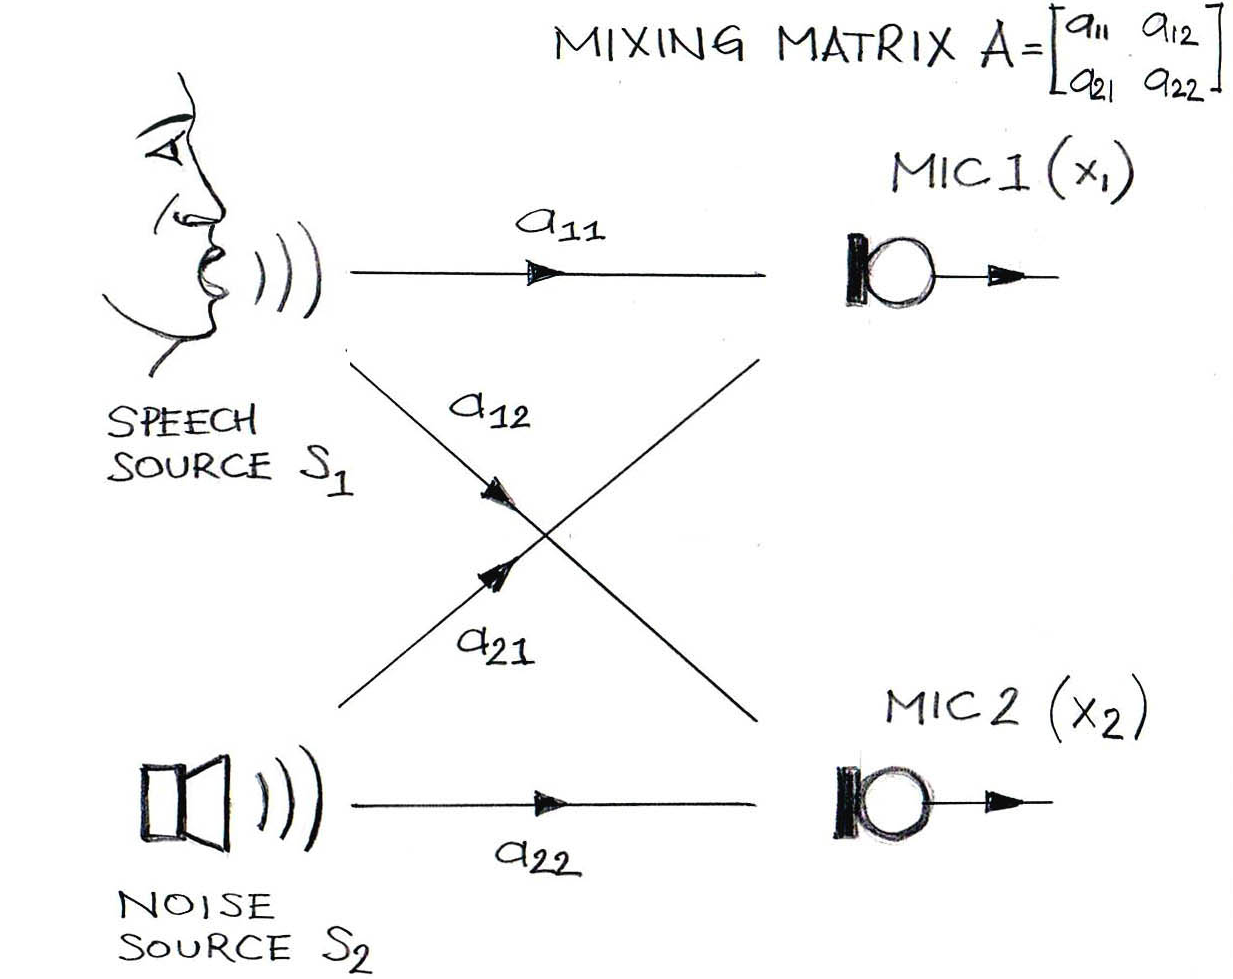
\includegraphics[scale=0.4]{two-sound-sources}
\end{center}


Stiind $x_1$ si $x_2$, daca am cunoaste elementele matricii $A$, atunci am putea afla $s_1$ si $s_2$ prin mijloace normale, fiind o ecuatie liniara. Dar, formuland problema ca mai inainte, informatiile initiale sunt cele 2 semmnale inregistrate de la cele 2 microfoane.

O abordare de rezolvare a problemei ar putea fi sa incercam sa ne folosim de proprietatiile statistice ale semnalelor $s_1(t)$ si $s_2(t)$ pentru a estima matricea $A$. Tot ce trebuie sa facem este sa presupunem ca semnalele $s_i(t)$ sunt independente statistic la fiecare moment $t$.

\subsection{Definitia riguroasa ICA}
Pornim de la presupunerea ca observam $n$ amestecari liniare $x_1, x_2, \ldots, x_n$ a $n$ componente independente:
	\begin{equation}
		x_j=a_{j1}s_1+a_{j2}s_2+\ldots+a_{jn}s_n, \text{ pentru toate }j.
	\end{equation}

Se observa ca am renuntat la indicele de timp $t$, deoarece ICA presupune ca atat fiecare amestecare $x_j$ cat si fiecare sursa $s_k$ sunt variable aleatoare, lucru care o sa fie folositor cand vom vorbi despre distributia datelor. De asemenea, ne vom asigura ca variabilele observate $x_j$ sunt centrate, scazand media esantioanelor.

Este convenient sa ne folosim de notatia vector-matrice, in locul sumelor precum cea precedenta. De acum vom nota \textbf{x} vectorul al carui elemente sunt amestecarile $x_j$, si la fel pentru \textbf{s}, ale carui elemente sunt $s_j$. De asemenea, vom nota \textbf{A} matricea de elemente $a_{ij}$. Folosind aceasta notatie, modelul de amestecare se scrie astfel:
\begin{equation}
	\textbf{x}=\textbf{As}.
\end{equation}

Modelul prezentat este modelul ICA, si este un model generativ, descris in statistica astfel:
\begin{equation}
	P(X|Y=y) 
\end{equation}
unde $X$ este o variabila observabila, iar $Y$ este variabila cautata, ceea ce inseamna ca descrie cum datele observate, $x_i$, sunt generate de un proces aplicat asupra datelor initiale, in cazul nostru componentele $s_i$. Componentele independente sunt variabile latente, nu sunt observate direct, ci sunt deduse din alte variable. De asemenea, presupunem ca matricea de amestecare $A$ nu este cunoscuta. Tot ce observam este vectorul aleator \textbf{x}, si trebuie sa estimam atat \textbf{A} cat si \textbf{s}. Acest lucru trebuie facut sub anumite ipoteze.

Punctul de inceput al ICA este ipoteza ca componentele independente $s_i$ sunt independente statistic, lucru pe care il vom defini mai incolo. Vom presupune deasemenea ca acestea au distributie \textbf{nongaussiana}, si ca matricea $A$ de amestecare este patrata. Dupa ce am estimat matricea $A$, ii putem calcula inversa, sa zicem \textbf{W}, si obtinem componentele independente astfel:
\begin{equation}
\textbf{s}=\textbf{Wx}
\end{equation}

\subsection{Limitarile ICA}
Avand in vedere modelul dat, se pot observa 2 limitari:

1. Nu putem determina \textbf{energiile} componentelor independente.

Motivul este ca, atat \textbf{s} cat si \textbf{A} sunt necunoscute, orice multiplicator scalar al unei dintre surse $s_i$ ar putea fi negat prin impartirea coloanei corespunzatoare $a_i$ al \textbf{A} cu acest scalar. Acelasi lucru se intampla cu semnul variabilelor, acesta se poate inmulti cu $-1$ fara a afecta modelul. Din fericire, aceasta limitare nu este semnificativa in majoritatea cazurilor.

2. Nu putem determina ordinea componentelor independente:

Motivul este ca, din nou, atat \textbf{s} cat si \textbf{A} fiind necunoscute, putem schimba ordinea termenilor din suma precedenta, oricare dintre componente putand fi prima. Formal, avand o matrice de permutare \textbf{P} si inversa ei, modelul poate fi formulat astfel:
\begin{equation}
	x=AP^{-1}Ps.
\end{equation}

Elementele lui \textbf{Ps} sunt componentele independente originale, dar in ordine diferita, iar matricea $\textbf{AP}^{-1}$ este doar o noua matrice de amestecare necunoscuta, care poate fi aflata.
\newpage

\subsection{Independenta}
\subsubsection{Definitie} 

Ca sa putem intelege conceptul de independenta, consideram 2 variabile scalare aleatoare, $y_1$ si $y_2$. Variabilele $y_1$ si $y_2$ sunt independente daca informatia din $y_1$ nu influnteaza informatia din $y_2$ si invers. Acest lucru este valabil pentru variabilele precedente $s_1,s_2$, dar nu si pentru amestecarile $x_1,x_2$.

Independenta poate fi definita prin probabilitati de densitate. O functie de densitate a unei probabilitati este folosita pentru a specifica probabilitatea unei variabile aleatoare de a avea valori dintr-un anumit interval. Probabilitatea este data prin integrarea functiei cu limitele intervalului. Sa notam $p(y-1,y_2)$ functia de densitate cumulata a $y_1$ si $y_2$, si $p_1(y_1)$ functia de densitate marginala a $y_1$, care reprezeinta functia de densitate a variabilei $y_1$:
\begin{equation}
p_1(y_1)=\int{p(y_1,y_2)dy_2},
\end{equation}
si similar pentru $y_2$. Acestea fiind spuse, definim $y_1$ si $y_2$ ca fiind independente daca:
\begin{equation}
	p(y_1,y_2)=p_1(y_1)p_2(y_2)
\end{equation}

Definitia aceasta poate fi folosita pentru a demonstra una dintre cele mai importante proprietati ale variabilelor aleatoare independente. Folosind functii $h_1$ si $h_2$ de mai sus, avem:
\begin{equation}
E{h_1(h_1),h_2(y_2)}=E{h_1(y_1)}E{h_2(y_2)}
\end{equation}
Putem demonstra astfel:
\begin{equation}
\begin{split}
E\{h_1(y_1),h_2(y_2)\} & =\iint{h_1(y_1)h_2(y_2)p(y_1,y_2)dy_1dy_2} \\ 
& =\iint{h_1(y_1)p_1(y_1)h_2(y_2)p_2(y_2)dy_1dy_2} \\
& =\int{h_1(y_1)p_1(y_1)dy_1}\int{h_2(y_2)p_2(y_2)dy_2}\\ 
& =E\{h_1(y_1)\}E\{h_2(y_2)\}
\end{split}
\end{equation}

\subsubsection{Corelatia si independenta}
O forma mai slaba de independenta este necorelatia. Doua variabile independente $y_1$ si $y_2$ se numeste necorelate daca covariatia lor este 0:
\begin{equation}
	E\{y_1y_2\}-E\{y_1\}E\{y_2\}=0
\end{equation}
Daca variabilele sunt independente, ele sunt necorelate, rezultand $h_1(y_1)=y_1$ si $h_2(y_2)=y_2$ din ecuatia precedenta.
Pe de alta parte, necorelarea nu implica independenta. Sa presupunem ca $(y_1,y_2)$ sunt valori discrete si au o distributie astfel incat perechea are $1/4$ sanse sa ia una dintre valorile urmatoare: $(0,1),(0,-1),(1,0),(-1,0)$. Atunci $y_1$ si $y_2$ sunt necorelate, dar:
\begin{equation}
E\{y_1^2, y_2^2\}=0 \neq \frac{1}{4} = E\{y_1^2\}E\{y_2^2\}
\end{equation}
si astfel conditia de mai sus nu este respectata, variabilele nefiind independente.
\subsubsection{Variabile nongaussiene}
Restrictia fundamentala a ICA este ca componentele independente sa fie nongaussiane pentru ca separarea sa se intample. Ca sa vedem de ce acest lucru este necesar, sa presupunem ca sursele $s_1, s_2$ au distributie gaussiana, iar $A$ este o matrice ortonormala. Din asta rezulta ca $x_1,x_2$ vor fi gaussiene, necorelate si au variatie unitara. Densitatea cumulata a $x_1, x_2$ este:
\begin{equation}
	p(x_1,x_2)=\frac{1}{2\pi}\exp(-\frac{x_1^2+x_2^2}{2})
\end{equation}

Distributia aceasta este ilustrata mai jos:
\begin{center}
	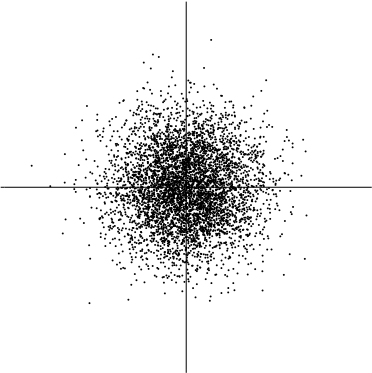
\includegraphics[scale=0.9]{multivariate_gaussian_distribution}
 \end{center}
 Se poate observa cum densitatea este complet simetrica. Asta inseamna ca nu contine informatii cu privire la directiile coloanelor matricii de amestecare $A$. Din acest motiv, $A$ nu poate fi estimat.

 \subsection{Principiile estimarii ICA}
 \subsubsection{Nongaussianitate inseamna independenta}
 Daca luam in calcul cele spuse pana acum, putem deduce ca esenta estimarii unui model ICA sta in nongaussianitate.

 Teorema limita centrala, in versiunea clasica, stabileste ca sumele partiale "normalizate" ale unui sir de variabile aleatoare independente si identic distribuite, cu dispersie finita, tind in distributie catre legea normala (gaussiana).\cite{paltanea}

 Sa presupunem ca datele din vectorul $x$ este distribuit asemenea modelului ICA prezentat mai devreme, adica ca o amestecare de componente independente, si distributia componentelor independente este  identica. Pentru a estima componentele independente, trebuie sa aplicam operatii liniare asupra $x_i$:
 \begin{equation}
	y=w^Tx=\sum_{i}w_ix_i, \text{unde $w$ este vectorul pe care il cautam.}
 \end{equation}

 Daca $w$ ar fi un rand al inversei lui $A$, aceasta combinatie liniara ar fi egala cu una dintre componentele independente. Ca sa vedem cum teorema limita centrala este folosita pentru a gasi un $w$ ca sa respecte conditia precedenta, putem face o schimbare de variabile, definind $z=A^Tw$. Apoi avem:
 \begin{equation}
	 y=w^Tx=w^TAs=z^Ts
 \end{equation}
 Se observa ca $y$ este o combinatie liniara de $s_i$, cu ponderile date de $z_i$. Deoarece suma suma celor doua variabile independente este mai gaussiana decat variabilele originale, $z^Ts$ este mai gaussian decat oricare $s_i$, si devine mai putin gaussian atunci cand este $s_i$, in acest caz, doar un element al lui $z$ este diferite de 0. 
 
 Cautam $w$ astfel incat $w^Tx$ sa fie cat mai nongaussian. Un astfel de vector ar corespunde unui $z$ care are doar o componenta diferita de zero. Asta inseamna ca $w^Tx=z^Ts$ este egal cu una dintre componentele independente.

 Maximizand nongaussianitatea lui $w^Tx$ ne da una dintre componentele independente. Spatiul de cautare pentru optimizarea nongaussianitatii intr-un spatiul $n$-dimensional al vectorilor $w$ are $2n$ maxime locale, 2 pentru fiecare componente independenta, $s_i$ si $-s_i$. Ca sa gasim mai multe componente independente, trebuie sa gasim toate maximele locale.  
\newpage
\subsection{Masuratori ale nongaussianitatii}
Pentru a folosi nongaussianitatea in estimarea ICA, avem nevoie de o masura cantitativa a nongaussinitatii unei variabile aleatoare, $y$. Vom presupune ca $y$ este centrat, adica are media egala cu zero, iar variatia ei este unu. 
\subsubsection{Aplatizarea}
O masura clasica a nongaussinitatii este aplatizarea (kurtosis), sau al patrulea moment central al unei variabile aleatoare, si este definit astfel:
\begin{equation}
kurt(y)=E\{y^4\}-3(E\{y^2\})^2
\end{equation}
Deoarece am stabilitia ca variatia este unu, atunci formula se simplifica la:
\begin{equation}
kurt(y)=E\{y^4\}-3
\end{equation}
Acest lucru arata defapt ca aplatizarea reprezinta al patrulea moment, $E\{y^4\}$. Pentru un $y$ gaussian, al patrulea moment este definit ca $3(E\{y^2\})^2$, deci aplatizarea pentru un asemenea $y$ este 0. Pentru majoritatea variabilelor aleatoare nongaussiene, aplatizarea este diferita de zero.

Aplatizarea poate fi pozitiva sau negativa, variabilele aleatoare care au aplatizare negativa numinduse subgaussiene, iar cele care au aplatizare pozitiva se numest supergaussiene. Variabilele aleatoare supergaussiene corespund cu distributii de tip Laplace, care au un varf ascutit, si coada alungita \cite{laplace_distribution_wiki}:
\begin{center}
	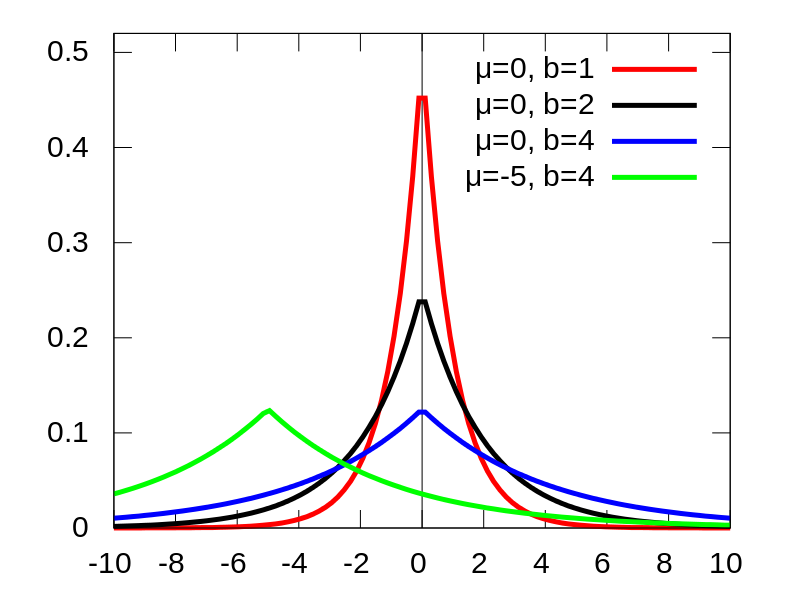
\includegraphics[scale=0.3]{laplace_distribution}
 \end{center}

 Variabilele aleatoare subgaussiene corespund cu distributiile uniforme, acestea fiind plate in reprezentare \cite{uniform_distribution_wolfram}:

\begin{center}
	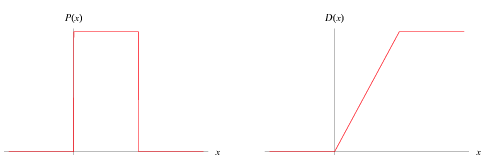
\includegraphics[scale=1.2]{uniform_distribution}
 \end{center}

Valoarea absoluta a aplatizarii, a fost folosita ca masura a nongaussianitatii in ICA, deoarece este simplu atat teoretic cat si computational. Pentru a calcula aplatizarea, putem folosi pur si simplu al patrulea moment al datelor avute. Analiza teoretica este simplificata datorita proprietatii de liniaritate. Daca avem doua variabile aleatoare independente, atunci:
\begin{equation}
kurt(x_1+x_2)=kurt(x_1)	+ kurt(x_2)
\end{equation}
\begin{equation}
kurt(\alpha x_1)=\alpha^4kurt(x_1)
\end{equation}

Pentru a demonstra cum arata spatiul de optimizare pentru aplatizare, si cum se pot afla componentele independente pot fi gasite prin maximizarea sau minimizarea aplatizarii. Avand modelul $x=As$ ca mai inainte, si componentele independente $s_1$ si $s_2$, cu valorile aplatizarii $kurt(s_1)$ si $kurt(s_2)$, ambele diferite de zero, cautam componentele independente prin $y=w^Tx$.
Facem din nou transformarea $z=A^Tw$. Apoi avem:
\begin{equation}
y=w^Tx=w^TAs=z^Ts=z_1s_1+z_2s_2
\end{equation}

Folosind proprietatiile aplatizarii mentionate mai devreme avem:
\begin{equation}
kurt(y)=kurt(z_1s_1)+kurt(z_2s_2)=z_1^4kurt(s_1)+z_2^4kurt(s_2)	
\end{equation}

Mai devreme am spus ca variatia lui $y$ este unu, deoarece $s_1$ si $s_2$ au variatia unu. Acest lucru implica faptul ca:
\begin{equation}
E\{y^2\}=z_1^2+z_2^2=1
\end{equation} 
ceea ce inseamna ca $z$ este restrans la un cerc cu raza unu in spatiul 2D. Problema de optimizare este urmatoarea: care este maximul functiei $|kurt(y)|=|z_1^4kurt(s_1)+z_2^4kurt(s_2)|$ pentru acest tip de cerc?

Maximele in acest caz sunt in punctele unde exact unul dintre elementele vectorului $z$ este zero si celalalt este diferit de zero, si deoarece ne aflam intr-un cerc cu raza unu, elementul diferit de zero este egal cu $-1$ sau $1$. Putem observa ca aceste puncte sunt cele in care $y$ este egal cu unul dintre componentele independente $\pm s_i$, si problema este rezolvata.

In practica am incepe de la un $w$ aleator, am calcula directia in care aplatizarea lui $y=w^Tx$ creste cel mai rapid, daca aplatizarea este pozitiva sau scade cel mai rapid, daca aplatizarea este negativa, in functie de esantioanele lui $x(i)$ al vectorului de mixturi $x$, si folosind o metoda de tip gradient pentru a gasi un nou vector $w$.

In practica, aceasta metoda are cateva dezavantaje. Aplatizarea este sensibila la valori extreme setului de date, ceea ce ar insemna ca toata aproximarea ar depinde de aceste valori, lucru care cauzeaza rezultate eronate.

\subsubsection{Neghentropia}
Neghentropia este a doua metoda foarte importanta pentru masurarea nongaussianitatii unor variabile aleatoare independente. Din punctul de vedere al teoriei informatiei, neghentropia se bazeaza pe cantitatea de entropie diferentiala. Conceptul de entropie este un concept de baza in teoria informatiei. Aceasta reprezinta gradul de informatie pe care observarea unei variabile o da. Cu cat variabila este mai putin structurata si mai putin previzibila, cu atat mai mare este entropia variabilei. Entropia $H$ a unei variabile aleatoare discrete $Y$ este:
\begin{equation}
	H(Y)=-\sum_i P(Y=a_i)log P(Y=a_i)
\end{equation}
unde $a_i$ reprezinta valorile posibile alea lui $Y$. Aceasta definitie poate fi generalizata pentru variabile aleatoare continue, in acest caz, numinduse entropie diferentiala:
\begin{equation}
H(Y)=-\int f(y) logf(y)dy	
\end{equation}
unde $f(y)$ este functia de densitate a unui vector aleator $y$.

Un rezultat fundamental al teoriei informatiei este stabilirea faptului ca variabilele gaussiene au cea mai mare entropie, comparativ cu alte variabile cu variatie egala. Asta inseamna ca entropia poate fi folosita ca si masura pentru nongaussianitate, aratand ca variabilele cu distributie gaussiana sunt cele mai putin structurate dintre toate distributiile. Entropia este mica pentru variabilele ale caror distributii sunt concentrate pe anumite valori, fiind analog unor functii cu varfuri ascutite, de tip Laplace. Pentru a obtine o masura a nongaussianitatii care este zero pentru o variabila aleatoare gaussiana si tot timpul pozitiva, se foloseste o versiune modificata a definitiei entropiei diferentiale, numita neghentropie. Neghentropia $J$ este definitia astfel:
\begin{equation}
	J(y)=H(y_{gauss})-H(y)	
\end{equation}
unde $y_{gauss}$ este variabila aleatoare gaussiana care are aceasi matrice de covariatie ca si $y$. Datorita proprietatilor de mai sus, neghentropia este pozitiva, si zero atunci cand variabila $y$ are distributie gaussiana. 

La fel ca la aplatizare, aproximarea neghentropiei are un dezavantaj major, acela ca este greu de calculat din punct de vedere computational, deoarece ar fi nevoie de o estimare a functiei de densitate, lucru care nu poate fi facut precis. 

\subsubsection{Aproximarea neghentropiei}
Dupa cum am mentionat mai devreme, aproximarea neghentropiei este dificila. In practica, se fac anumite aproximari, iar tipurile de aproximari abordate se va face aici. 
\begin{equation}
	J(y)\approx \frac{1}{12}E\{y^3\}^2 + \frac{1}{48}kurt(y)^2
\end{equation}
Prima abordare este cea bazata pe momentele statistice:
Variabila $y$ se presupune ca are media egala cu zero, si variatie unitara. Se poate observa ca aceata abordare sufera de aceleasi limitari precum aproximarea folosind aplatizarea. Pentru a evita acest lucru, s-au dezvoltat aproximari bazate pe principiul entropiei maxime, cu forma:
\begin{equation}
	J(y)\approx\sum_{i=1}^p k_i[E\{G_i(y)\}]-E\{G_i(v)\}]^2
\end{equation}
unde $k_i$ reprezinta constante pozitive, si $v$ este o variabila gaussiana, iar atat $v$ cat si $y$ au media zero si variatie unitara, functiile $G_i$ fiind niste functii nonpatratice. In cazul in care folosim o singura functie nonpatratica, aproximarea devine:
\begin{equation}
	J(y)\propto[E\{G(y)\}]-E\{G(v)\}]^2
\end{equation}
Alegand $G$ bine, putem obtine aproximari mult mai bune decat cele de mai devreme, spre exemplu, daca alegem $G$ care nu creste repede, precum:
\begin{equation}
	G_1(u)=\frac{1}{a_1}\log \cosh a_1 u_1, G_2(u)=-\exp(\frac{-u^2}{2})
\end{equation}
unde $1\leq a_1 \leq 2$ este o constanta. Cu toate ca nu am folosit aceste tipuri de aproximari, ele sunt un compromis bun intre metodele de masurare a nongaussianitatii abordate mai devreme, aplatizarea si neghentropia. 

\subsection{Abordarea Maximum Likelihood}
O abordare foarte populara pentru rezolvarea modelului ICA este \textbf{maximum likelihood estimation}. Aceasta metoda estimeaza valorile parametrului unui model.\cite{probability_concepts} Acesti parametri sunt gasiti astfel inca estimarea lor sa mareasca sansa ca modelul sa produca datele observate. Pentru cazul particular al modelului nostru ICA, avand $W=(w_1, \dots, w_n)^T$ ca $A^{-1}$, \textbf{log-likelihood-ul} ia forma:
\begin{equation}
	L=\sum_{t=1}^T \sum_{i=1}^n \log f_i(w_i^Tx(t)) + T \log |\det W|
\end{equation}
unde $f_i$ este functia de densitate a lui $s_i$, aici presupunand ca o stim, iar $x(t)$ reprezinta esantioanele amestecarilor $x_i$. Termenul $\log | \det W|$ vine din faptul ca pentru un vector aleator $x$ cu densitatea $p_x$, si pentru orice matrice $W$:
\begin{equation}
	y=Wx, \text{data de } p_x(Wx)|\det W|.
\end{equation}

\subsection{Metoda Gradient Descent}
Metoda gradient descent este una dintre cele mai folosite metode pentru aproximarea maximului sau minimului pentru o functie complexa. Acesta functioneaza facand pasi in directia gradientului functiei in punctul curent, astfel se ajunge la minimul functiei. Daca in schimb, pasii sunt in directia pozitiva gradientului, se ajunge la maximul functiei. Gradientul unei functii reprezinta derivata partiala a functiei pe care incercam sa o minimizam sau maximizam.\cite{gradiend_descent_wiki}

Vom folosi aceasta metoda pentru a incerca sa aproximam matricea $A^{-1}$, sau $W$, aceasta fiind matricea care ne va ajuta sa separam componentele, asa cum am mentionat pana acum. Functia de update pentru o abordare de tip gradient descent pentru optimizarea maximum likelihood este:
\begin{equation}
	W^+=W+ \mu [I + g(y) y^T]W
\end{equation}
unde $\mu$ este rata de invatare a algoritmului, iar $g$ este functia de densitate a componentelor independente.\cite{hyvarien}

Un factor important in succesul acestui algoritm este alegerea functiei de densitate. Pana acum am presupus ca se cunoaste functia de densitate a componentelor independente, dar in practica, acest lucru nu poate fi garantat, iar din aceasta cauza, va fi nevoie de o aproximare. S-a observat ca o functie potrivita acestei probleme este functia sigmoida, deoarece avand o distributie continua, calculand derivata acestei functii ajungem la o functie de densitate, care poate fi folosita pentru aproximarea densitatii componentelor independente. Aici vom defini $g$ ca fiind functia sigmoida, in practica s-a demonstrat ca este suficient de buna:
\begin{equation}
	g_i(x)=\frac{1}{1+e^{-x}}
\end{equation}

Functia sigmoida are urmatoarea distributie \cite{sigmoid_function_wiki}:
\begin{center}
	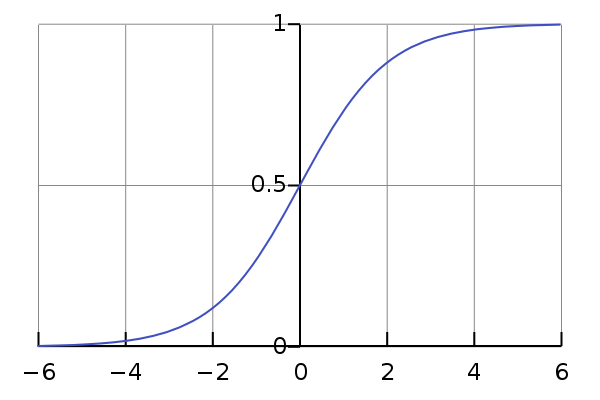
\includegraphics[scale=0.6]{sigmoid_function}
 \end{center}

\subsection{Metodologia si algoritmul}
\subsubsection{Jupyter Notebook}
Implementarea algoritmului s-a facut in limbajul de programare Python, folosind platforma Jupyter Notebook. Am ales aceasta platforma deoarece face ca pasii algoritmului sa poata fi mai bine urmariti, iar afisarea rezultatelor sa se faca intr-o maniera usoara si concisa. Aplicatia functioneaza pe un server local, iar codul este scris intr-un \textbf{notebook (caiet)}, prezent intr-o pagina web, codul fiind impartit in \textbf{cells (celule)}, in fiecare celula putem scrie o bucata de cod, care mai apoi poate fi executata. Acest stil de lucru este de folos deoarece permite executarea fiecarei celule individual, scurtand timpul dedicat intretinerii caietului. De asemenea, in aceste celule putem amplasa grafice, histograme, elemente de tip \textbf{mark-up} pentru prezentarea unor informatii suplimentare, si elemente de tip audio sau video. 

Pentru a executa testele prezentate aici, tot ce trebuie facut este deschiderea fisierului corespunzator testului in interfata Jupyter Notebook, si executarea tutoror celulelor din fisier.

\subsubsection{Semnalele audio testate}
Pentru testarea algoritmului, am ales mai multe seturi de semnale audio, fiecare cu proprietati diferite. Astfel, am realizat patru teste:
\begin{itemize}
	\item{Semnale primitive: pentru inceput, am testat algoritmul pe doua tipuri de semnale primitive, generate in notebook, unul de tip sinus, si unul de tip fierastrau.\cite{scikit_ica_pca}}
	\item{Voce si muzica: pentru a testa un caz de separare unde se poate face clar distinctia intre cele doua semnale amestecate, am ales o voce care spunea cifrele in engleza, si o melodie.\cite{sound_samples_1}
} 	\item{Doua voci: acesta a fost testul care simula cel mai bine realitatea, doua voci, una care spunea cifrele in engleza, si una care spunea cifrele in spaniola.\cite{sound_samples_1}} 
	\item{Trei semnale: acesta a fost testul care demonstra faptul ca se pot separa mai mult de doua componente independente amestecate, asa cum era ipoteza in teorie. Semnalele alese au fost cele reprezentand un aspirator in functiune, o voce umana, si un grup de oameni ce aplauda.\cite{vsubhashini}}
\end{itemize}

\subsubsection{Pre-procesarea datelor}
Pentru toate semnalele audio inafara de cele primitive, a fost nevoie sa centram datele, la fel ca in cazul PCA, pentru standardizare. 

Pornind de la semnalele audio initiale, vom simula amestecarea lor, folosind operatorul de amestecare, $A$. In realitate, acest $A$ ar fi dat de distantele dintre sursele de semnal si dispozitivele care le inregistreaza. In cazul nostru, $A$ va fi o matrice patratica, fie de $2 \times 2$, fie de $3 \times 3$, in functie de caz. Acest proces arata ca mai inainte \cite{noise_reduction}:
\begin{center}
	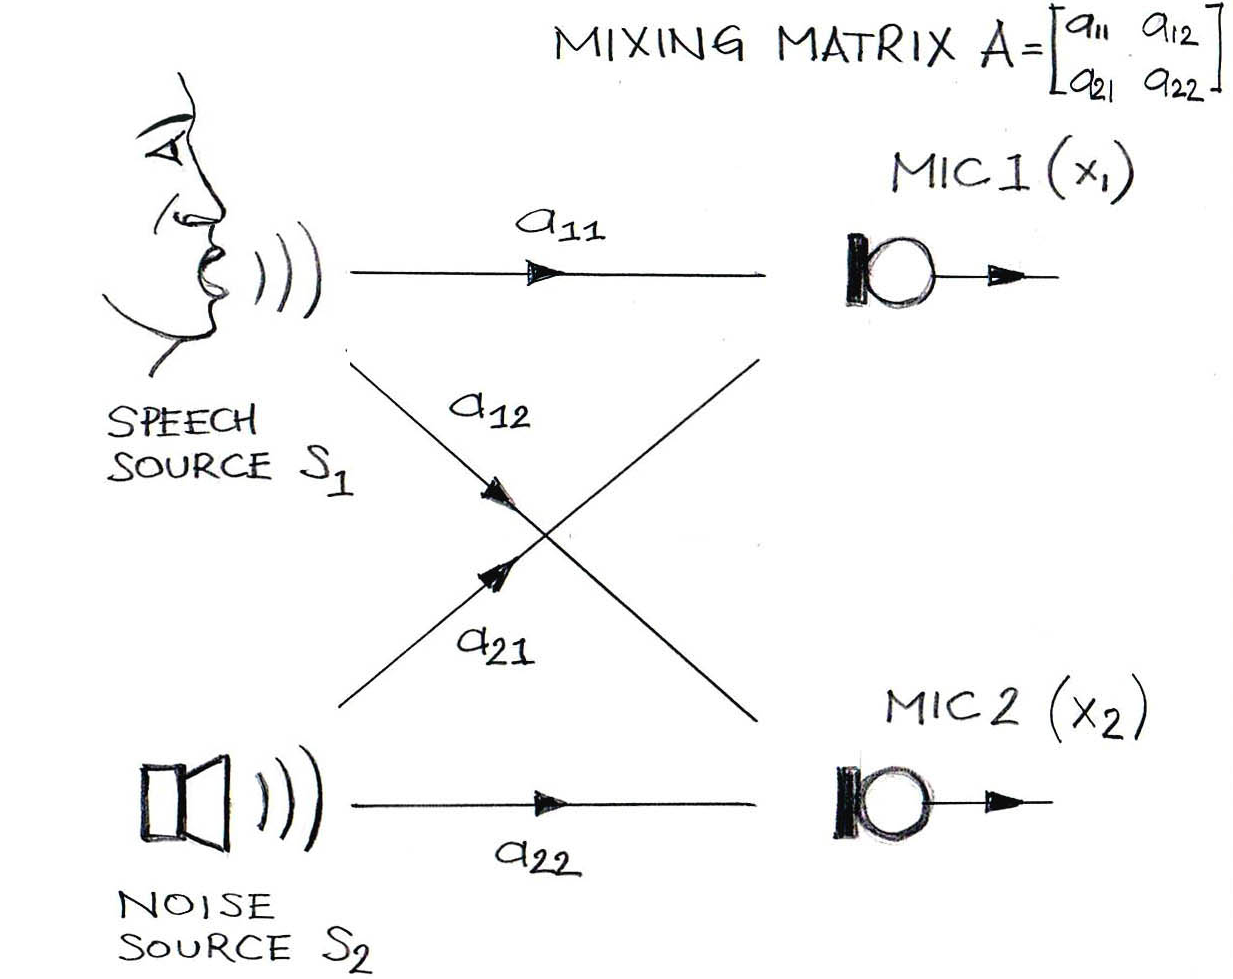
\includegraphics[scale=0.3]{two-sound-sources}
 \end{center}

Pentru fiecare caz testat, am ales initial matricea $A$ aleator, cu valorile distribuite uniform intre $0.01$ si $0.1$. Deoarece acest lucru a facut verificarea rezultatelor si modificarea algoritmului destul de greu, am ales dintre matricile aleatoare $A$ cele care au demonstrat cel mai bine eficacitatea algoritmului. O astfel de matrice este:
\[
 \begin{matrix}
 	0.56804456  & 0.92559664 \\
	0.07103606  & 0.08712930 
 \end{matrix}
\]
Vom prezenta mai tarziu rezultatele fiecarui test, iar acolo vor fi prezentate toate variabilele folosite pentru a se ajunge la rezultatele noastre.

\subsubsection{Aplicarea algoritmului Gradient Descent}
Implementarea folosita a fost o adaptare in limbajul Python a unei cercetari facute in limbajul Matlab.\cite{vsubhashini} Avand sursele de semnal amestecate, trebuie sa aplicam algoritmul gradient descent prezentat mai devreme pentru a incerca sa gasim componentele independente initiale.  Pentru acest lucru, vom porni de la o matrice $A^{-1}$, sau $W$, cu valori aleatoare uniform distribuite intre $0.01$ si $0.1$. Acest interval s-a observat ca fiind unul bun pentru cazurile noastre, dar el trebuie adaptat in functie de situatie. 

Se calculeaza:
\begin{equation}
	Y=WX
\end{equation} 
unde $Y$ reprezinta banuiala algoritmului cu privire la componentele independente. Functia de actualizare a lui $W$, definita mai sus, va gasi un $W$ mai bun, luand in calcul $Y$. In faza initiala, acest pas se executa pentru un numar finit de pasi, ales in functie de situatie, iar dupa fiecare iteratie rata de invatare se modifica prin metoda recoacerii simulate, asta inseamnand ca fiecare iteratie succesiva are o rata de invatare mai mica, simuland cautarea pe un spatiu de cautare mai mic, scazand posibilitatea ajungerii intr-un minim sau maxim local. Dupa terminarea executarii acestui numar de iteratii, $W$ actualizat ar trebui sa fie cel care poate sa separe componentele. Acest lucru nu este intotdeauna adevarat, ceea ce inseamna ca ne trebuie o alta metoda de a opri cautarea solutiei optime.

\subsubsection{Conditia de oprire}
Algoritmii care aplica metoda gradient descent, deobicei sunt opriti atunci cand functia de cost ajunge sau este foarte aproape de minim. In general, se considera ca functia a ajuns la costul minim atunci cand diferentele dintre valorile consecutive obtinute de algoritm sunt mai mici decat un anumit \textbf{threshold (prag)}. Alegere acestui prag este foarte importanta, deoarece un prag prea mic va duce la castiguri foarte mici de precizie dupa multe operatii, iar un prag mare poate va opri algoritmul inainte de a ajunge la valoarea minima. Cu toate ca aceasta idee pare destul de simpla, balansul dintre precizia rezultatului obtinut si viteza algoritmului este ceva ce trebuie masurat si ajustat de la caz la caz. Functia de cost calculata este:
\begin{equation}
	f_{cost}=\log g(Y)(1-g(Y))
\end{equation}
care va fi o matrice patratica, cu numarul de linii egal cu numarul de esantioane al lui $Y$. Pentru ca trebuie sa calculam diferenta dintre costurile iteratiilor consecutive, si pentru ca nu putem face asta usor pentru matrici, vom modifica functia de cost astfel incat ea sa devina suma elementelor matricii rezultate din functia $f_{cost}$.

Aceasta abordare este cea de preferat in cazul algoritmilor de tip gradient descent, deoarece avem un mod obiectiv de a masura performanta algoritmului, si pentru ca functia de cost este legata direct de restul operatiilor. In realitate, am descoperit ca metoda aceasta de a opri algoritmul nu este posibila atunci cand lucram cu semnale audio lungi, care pot avea pana la 16000 de esantioane pe secunda, matricea pentru care trebuie sa calculam suma elementelor ar avea dimensiuni foarte mari, spre exemplu $120000 \times 120000$ elemente, care nu incape in memoria RAM a calculatorului. 

O alta abordare pentru a masura independenta este necorelatia, asa cum am mentionat intr-un capitol precedent. Acolo am spus ca daca doua variabile sunt independente, ele sunt necorelate, dar afirmatia inversa nu este intotdeauna adevarata. Deoarece abordarea care implica functia de cost nu era potrivita pentru semnale audio de dimensiuni mari, pentru testele care implicau acest tip de componente, am decis sa folosim necorelatia pentru a masura independenta componentelor. Dupa fiecare iteratie a algoritmului, am calculat corelatia intre componentele rezultate, si daca se afla sub un anumit prag, deobicei foarte mic, spre exemplu $3e^{-6}$. Aceasta abordare s-a dovedit a fi una reusita, era consistenta de-a lungul testelor, si poate fi aplicata pentru orice fel de semnale. 

\subsubsection{Implementarea algoritmului}
\begin{lstlisting}[language=Python]
def sigmoid(y):
    g=np.divide(1,np.add(1,np.exp(-y)))
    return g

def gradient(eta, Y, W):
    Z=sigmoid(Y)
    Id=np.identity(Y.shape[0])
    grad=eta*(Id+np.dot((1-2*Z),Y.T))*W
	return grad

corr=1
while abs(corr)>=4e-6:
	eta=0.01
	eta0=eta
	T=1000
	num_iter=10000
	W=np.random.uniform(0.001,0.01,(n,n))
	for i in range(0,num_iter):
		Y=np.dot(W,X)
		delW=gradient(eta,Y,W)
		W+=delW
		eta=eta0/(1+(i/T))
	Y2=np.dot(W,X)
	corr=np.corrcoef(Y2)[1][0]

Y2=np.dot(W,X)
\end{lstlisting}
Constantele alese aici sunt particulare pentru testul cu muzica si vorbit.

\newpage
\subsection{Rezultate}
Dupa cum am mentionat mai sus, am realizat patru teste. Le vom prezenta aici pe fiecare, impreuna cu rezultatele obtinute.

\subsubsection{Semnale primitive}
Primul test a fost realizat cu doua semnale generate prin intermediul codului Python, unul de tip sinus, si unul de tip fierastrau:
\begin{center}
	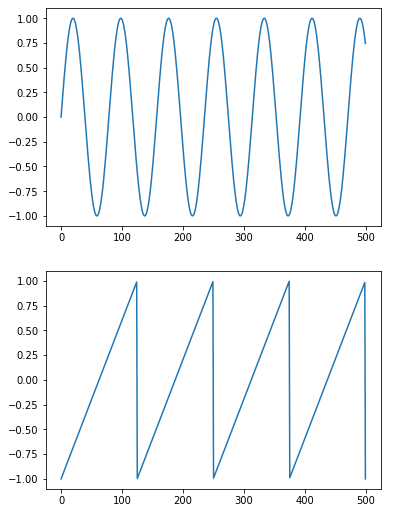
\includegraphics[scale=0.8]{primitive_waves}
\end{center}

Matricea de amestecare $A$ aleasa a fost:
\[
 \begin{matrix}
 	0.56804456  & 0.92559664 \\
	0.07103606  & 0.08712930 
 \end{matrix}
\]
Realizarea acestei amestecari arata astfel:
\begin{center}
	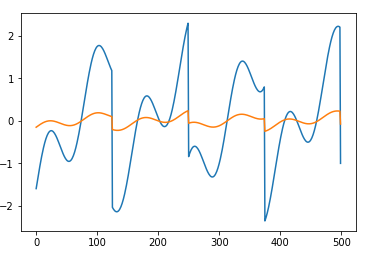
\includegraphics[scale=1]{primitives_mixed}
 \end{center}

Am ales aceasta prezentare a semnalelor deoarece se poate observa cum nu se poate distinge diferenta dintre semnalele initiale, desi se pot observa asemanari cu acestea, precum varfurile ascutite ale semnalului de tip fierastrau si curbele semnalului sinus. 

Dupa executarea algoritmului pe semnalele amestecate, se ajunge la urmatoarea separare:
\begin{center}
	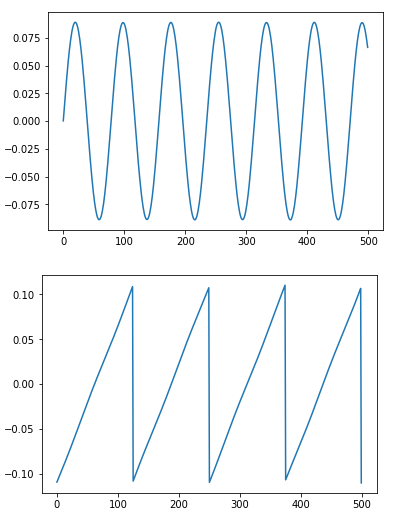
\includegraphics[scale=1]{primitives_separated}
 \end{center}

Se poate observa cum semnalele au fost complet separate, lucru care ne indica ca teoria prezentata pana acum este corecta. Coeficientul de corelatie al semnalelor separate este $0.000515439559418$. Pentru acest caz simplu, ICA isi face treaba foarte bine, iar timpul de executie este acceptabil, pana in 10 secunde.

\subsubsection{Semnale audio: voce si muzica}
Urmatorul test a fost efectuat cu doua semnale audio preluate de pe disc. Un semnal continea muzica, si un semnal continea o voce de barbat care spunea cifrele in engleza:
\begin{center}
	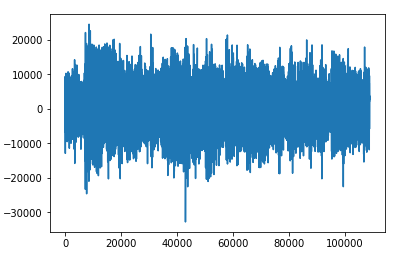
\includegraphics[scale=1]{music_music}
\end{center}
\begin{center}
	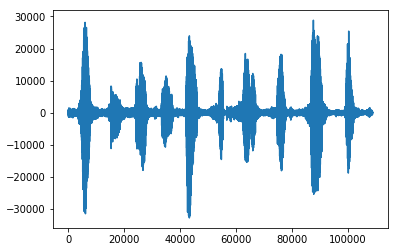
\includegraphics[scale=1]{speech_music}
\end{center}

Matricea de amestecare $A$ a fost:
\[
 \begin{matrix}
	0.15270211 & 0.08406566 \\
	0.90514896 & 0.53725471
 \end{matrix}
\]
Semnalele amestecate rezultate sunt:
\begin{center}
	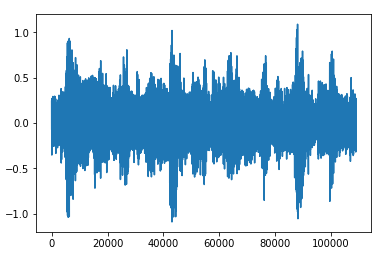
\includegraphics[scale=1]{music_mixed_1}
 \end{center}
\begin{center}
	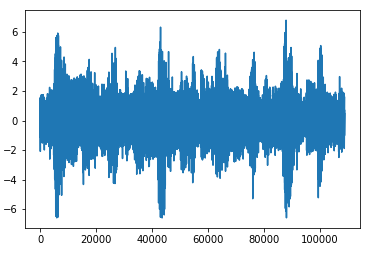
\includegraphics[scale=1]{music_mixed_2}
 \end{center}
 Am ales prezentarea lor separata deoarece avand magnitudini diferite, al doilea semnal l-ar fi acoperit pe primul in cazul unei afisari combinate. Acest caz de amestecare ar simula un caz din viata reala in care unul dintre microfoane este mai aproape de cele doua surse de semnal, iar celalalt mai departe. Se observa cum cele doua semnale sunt aproape identice, daca ignoram factorul magnitudinii. 

 Rezultatele separarii:
\begin{center}
	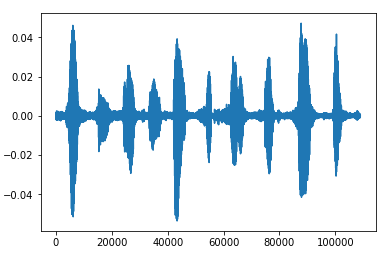
\includegraphics[scale=1]{music_separated_1}
 \end{center}
\begin{center}
	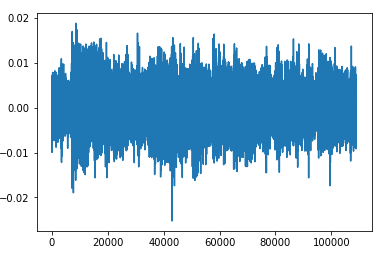
\includegraphics[scale=1]{music_separated_2}
 \end{center}

 Din nou, se observa o separare foarte buna semnalelor amestecate, coeficientul de corelatie fiind $-3.11671198288e-06$, acest exemplu fiind foarte expresiv in acest sens, se poate face foarte clar diferenta dintre semnalul cu voce si cel cu muzica. 

 \subsubsection{Semnale audio: doua voci}
 Urmatorul este a fost efectuat cu doua semnale audio, ambele contineau voci de barbat, unul spunea cifrele in engleza, iar celalalt spunea cifrele in spaniola:
 \begin{center}
	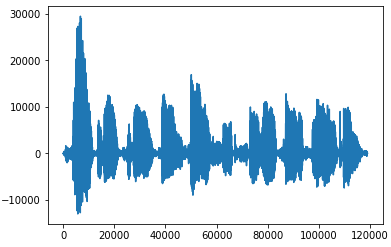
\includegraphics[scale=1]{english_speech}
 \end{center}
\begin{center}
	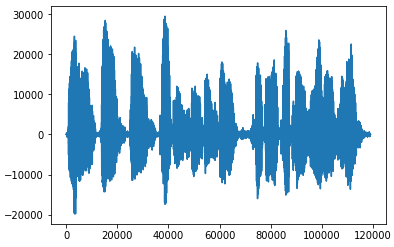
\includegraphics[scale=1]{spanish_speech}
\end{center}
 
 Matricea de amestecare $A$ este: 
\[
 \begin{matrix}
	0.82583118 & 0.39868634 \\
	0.12657259 & 0.96097025
 \end{matrix}
\]
Rezultatul amestecarii este:
\begin{center}
	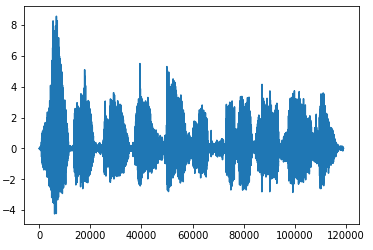
\includegraphics[scale=1]{speech_mixed_1}
 \end{center}

\begin{center}
	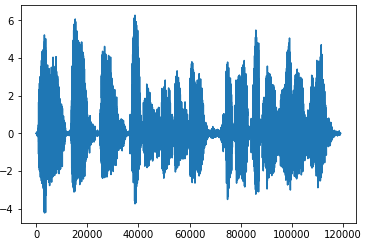
\includegraphics[scale=1]{speech_mixed_2}
 \end{center}

 Aceasta amestecare simuleaza un caz din viata reala cand primul microfon se afla la o distanta echidistanta de cele doua surse de semnal, iar al doilea microfon se afla mai aproape de semnalul cu vocea spaniola, pe fundal auzindu-se si vocea engleza.

Rezultatul separarii este:
\begin{center}
	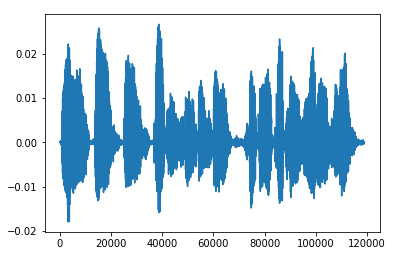
\includegraphics[scale=1]{speech_separated_1}
 \end{center}
\begin{center}
	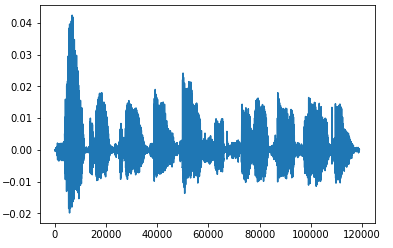
\includegraphics[scale=1]{speech_separated_2}
 \end{center}

 Coeficientul de corelatie al surselor separate este $5.62035243305e-08$, un coeficient foarte mic, care arata o separare buna, acest lucru se observa si din imagini, se poate face clar diferenta intre cele doua voci, si se vede asemanarea cu semnalele originale. De asemenea, se poate vedea ca algoritmul nu pastreaza ordinea componentelor initiale, ele ies din algoritm in ordine inversa, lucru sustinut de teorie.

 \subsubsection{Semnale audio: trei semnale}
 Acest test a fost facut pentru a demonstra faptul ca ICA poate separa mai mult de doua surse independente, si a fost realizat cu trei semnale audio: un aspirator in functiune, o serie de aplaude si o voce:
\begin{center}
	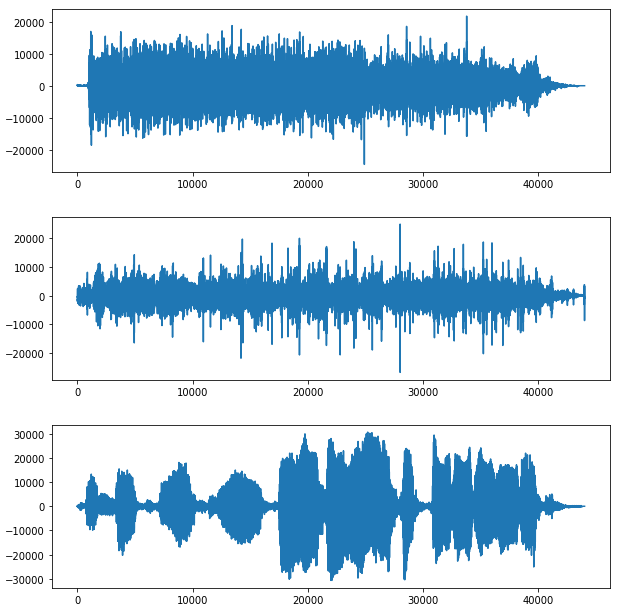
\includegraphics[scale=1]{three_initial}
 \end{center}

 Matricea de amestecare $A$ este:
\[
 \begin{matrix}
	0.77191 & 0.4752 &  0.58699 \\
	0.33712 & 0.47563 & 0.20836 \\
	0.96878 & 0.57618 & 0.65625
 \end{matrix}
\]
Rezultatul amestecarii este:
\begin{center}
	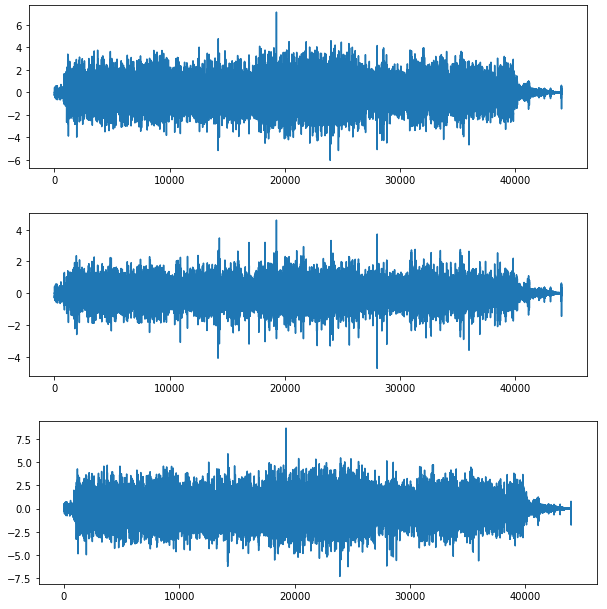
\includegraphics[scale=1]{three_mixed}
 \end{center}

 La fel ca in testele de pana acum, amestecarea rezulta in semnale care sunt foarte similare. Dupa executarea algoritmului, semnalele separate rezultate sunt:
\begin{center}
	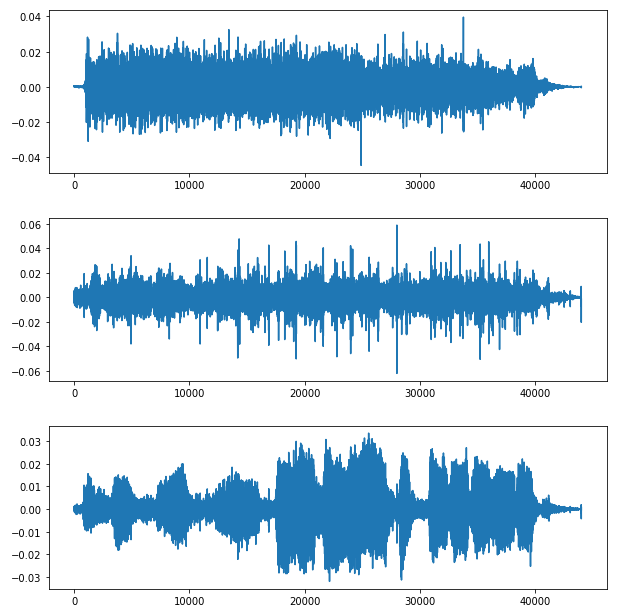
\includegraphics[scale=1]{three_separated}
 \end{center}

\subsubsection{Analiza coeficientilor de corelatie a testelor}
Uitandu-ne la coeficientii de corelatie ale surselor separate, se poate observa ca necesitatea ca ei sa fie mai mici, pentru o separare mai buna, creste, si asta deoarece complexitatea surselor amestecate este mai mare. Daca pentru semnalele primitive a rezultat un coeficient de corelatie de ordinul $5e^{-4}$, pentru semnalele audio reale acesta a fost si mai mic, $3e^{-6}$ in cazul muzicii amestecate cu voce, si $5e^{-8}$ in cazul vocilor amestecate. Asta arata ca cu cat semnalele initiale sunt considerate mai \textbf{asemanatoare} (putem spune ca doua voci sunt mai asemanatoare decat o voce si o melodie acustica), cu atat indicele de corelatie al semnalelor separate este mai mic.

\subsubsection{ICA versus PCA}
Deoarece am abordat si tema PCA in aceasta lucrare, am dorit sa efectuam un test in care comparam puterea de separare dintre ICA si PCA, in contextul componentelor independente. Din fericire, cei care au realizat biblioteca scikit-learn pentru Python au efectuat aceasta comparatie pentru noi.\cite{scikit_ica_pca} Acestia au folosit implementarile lor pentru algoritmii PCA si ICA, si deoarece am demonstrat ca implementarile noastre functioneaza conform teoriei, am decis ca nu mai este necesar sa efectuam acest test si cu algoritmii nostrii. Acestea sunt rezultatele:
\begin{center}
	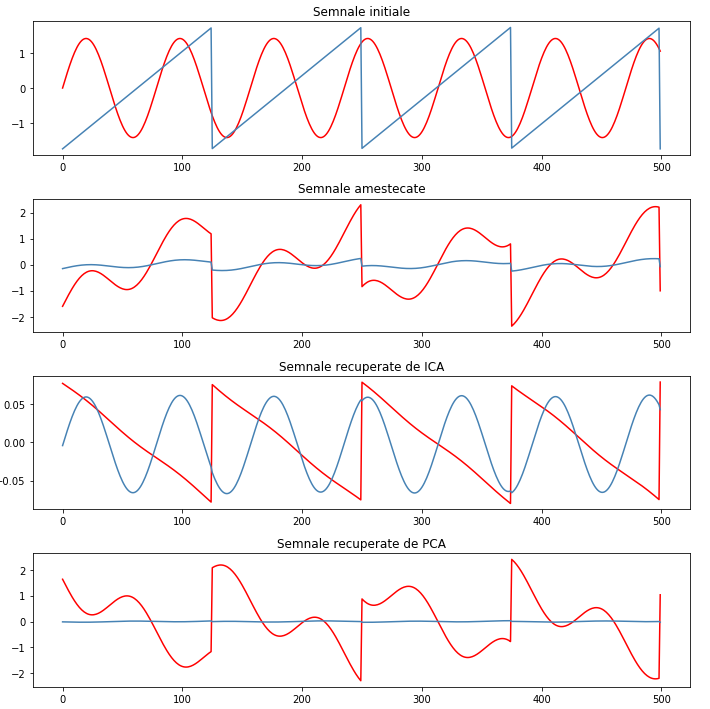
\includegraphics[width=\linewidth]{pca_vs_ica}
 \end{center}

 Se poate observa cum abordarea PCA nu reuseste sa separe componentele independente, in asemenea cazuri, abordarea ICA este mai buna.

\subsubsection{Problema ICA in lumea reala}
Pana acum, ipoteza teoriei descrise a fost faptul ca semnalele sunt amestecate instant, in diferite proportii. Acest lucru in lumea reala ar insemna ca semnalele audio pornesc de la sursa si ajung la receptori instant, luandu-se in calcul distanta. Se poate observa clar problema: in lumea reala exista un timp de parcurgere al semnalului, care variaza atat in functie de distanta dintre surse si receptori, cat si in functie de tipul mediului prin care se face propagarea. Aceasta intarziere poate fi de la mai putin de o milisecunda, pana la mai multe milisecunde. Avand in considerare faptul ca o secunda inregistrata de un receptor audio poate contine 16000 de esantioane, o intarziere de o milisecunda intre ajungerea unui semnal la cei doi receptori duce la o defazare de 16 esantioane intre inceputul inregistrarilor semnalului. Aceasta diferenta este destul de mare incat rezultatul obtinut de algoritm sa nu fie cel dorit. 

Testul efectuat pentru a ajunge la aceasta concluzie este urmatorul: am pornit de la doua semnale amestecate in conditii reale, muzica si o voce umana, si preluate de doua microfoane.\cite{sound_samples_1} Semnalele inregistrate sunt:
\begin{center}
	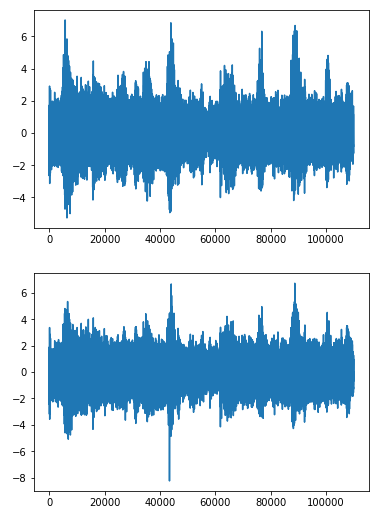
\includegraphics[scale=1]{real_mixed}
 \end{center}

 Dupa aplicarea ICA asupra acestor surse, se obtin urmatoarele semnale:
\begin{center}
	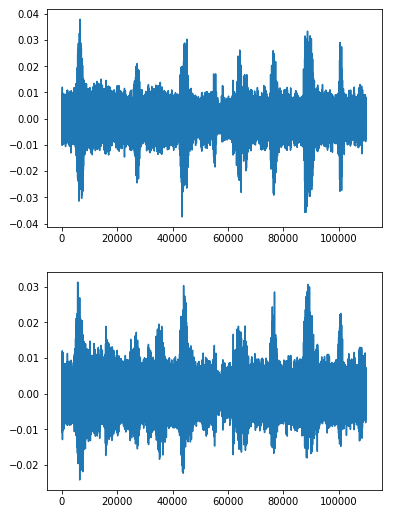
\includegraphics[scale=1]{real_separated}
 \end{center}

 Se poate observa ca nu s-a schimbat aproape nimic in configuratia semnalelor, ele ramanand amestecate, ICA fiind sensibil la defazarea semnalelor.

 Pentru a rezolva aceasta problema, se pot aplica doua solutii:
 \begin{itemize}
	\item{Se poate face o calibrare a microfoanelor, sau mai bine spus, a semnalelor primite, astfel incat atunci cand semnalele initiale ajung la microfon sa fie inregistrate digital cu intarzierea deja luata in calcul. Acest lucru s-ar putea face cu doua semnale scurte ascutite care pleaca din locul de unde vor pleca semnalele initiale care se vor amesteca, masurand intarzierea initiala cu ajutorul acestor semnale ascutite si apoi facand pre-procesarea pe semnalele amestecate.} 
	\item{A doua abordare este una matematica, daca in functia de maximum likelihood a algoritmului am putea lua in calcul intarzierea dintre semnale, fara ca intarzierea sa fie masurata in prealabil. Acest lucru ar insemna ca functia noua sa ia practic in calcul faza semnalelor, ceea ce ar duce problema in domeniul complex.}
 \end{itemize}

\subsection{Utilizari ale ICA} 

Aceste utilizari sunt prezentate conform articolului publicat de Aapo Hyvärinen si Erkki Oja.\cite{hyvarien}

\subsubsection{Separarea artefactelor din inregistrari MEG}
Magnetoencefalografia (MEG) este o procedure neinvaziva in care este monitorizata activitatea neuronilor corticali cu o precizie foarte buna din punct de vedere al timpului, si cu precizie moderata din punct de vedere spatial. Cand se analizeaza date MEG, o problema comuna este extractia caracteristicilor semnalelor neuromagnetice in prezenta artefactelor. Amplitudinea artefactelor ar putea fi mai mare decat cele ale semnalelor creierului, acestea putand fi interepretate ca semnale patologice, adica ca semnale care pot cauza sau descriu o anumita afectiune.

O posibila rezolvare a acestei probleme este considerarea faptului ca activitatea cerebrala si artefactele, fie ele miscari ale ochilor sau senzori defecti, sunt procese separate din punct de vedere anatomic si fiziologic, si aceasta separare este data de independenta statistica dintre semnalele magnetice generate de aceste procese.

Semnalele MEG au fost inregistrate intr-o camera izolata magnetic, cu un neuromagnetometru \textbf{Neuromag-122} cu 122 de canale, care acopera intreg scalpul pacientului. Aparatul inregistreaza date din 61 de locatii. Persoana de test a fost rugata sa clipeasca si sa faca miscari rapide si bruste cu ochii, pentru a produce artefacte oculare tipice. Pentru a produce artefacte musculare, acesta a fost rugat sa muste in gol, pana la 20 de secunde. Pe langa asta, un alt artefact a fost creat plasand un ceas digital la un metru de casca, inauntrul camerei izolate.

\begin{center}
	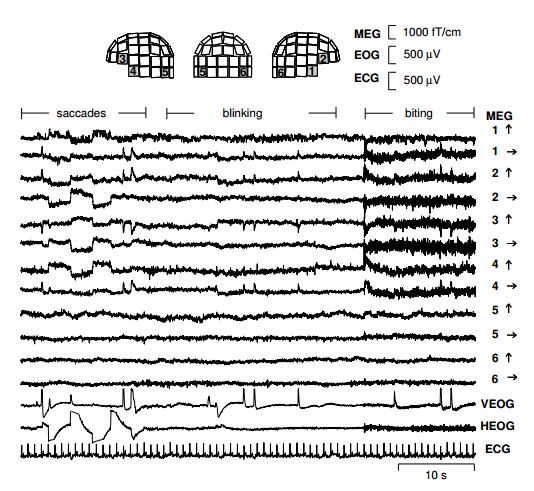
\includegraphics[scale=1]{meg_1}
 \end{center}
 In aceasta imagine\cite{hyvarien} se pot vedea 12 semnale MEG din zona frontala, temporala si occipitala, impreuna cu pozitia senzorilor pe casca. Ultimele trei semnale reprezinta doua electrooculograme si o electrocardiograma, si nu au fost folosite in prelucrarea datelor cu ICA.

 Asupra vectorului de semnale $x$, care contine amplitudinile $x(t)$ a 122 de semnale (deci dimensionalitatea este $n=22$), s-a aplicat mai intai PCA, pentru a reduce dimensionalitatea si pentru a standardiza datele. Apoi s-a aplicat un algoritm de tip ICA, rezultatele fiind urmatoarele\cite{hyvarien}:
\begin{center}
	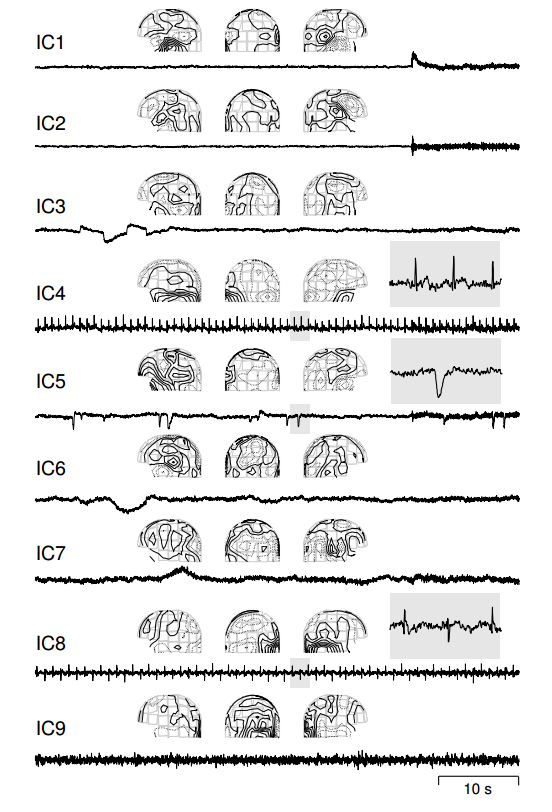
\includegraphics[scale=0.8]{meg_2}
 \end{center}
 In aceasta imagine se vad sectiuni de semnale pentru 9 dintre componentele independente rezultate dupa aplicarea ICA asupra setului de date. In primele doua componente independente au aparut din cauza activitatii musculare cauzate de muscat. Aceasta separare in doua componente pare sa corespunda celor doua seturi de muschi care au fost activati in timpul procesului. A treia si a cincea componenta independenta arata miscarile bruste si rapide ale ochilor, impreuna cu clipitul aferent. A patra componenta arata artefactul cardiac care a fost extras. Ultimele doua componente independente, IC8 si IC9 au fost obtinute dupa o filtrare superioara a frecventelor de peste 1 Hz, IC8 arata artefactele date de ceasul din camera izolata, iar IC9 arata un senzor care are un sunet de fundal mai mare decat restul senzorilor. 

 Acest test arata cum ICA este folosit in separarea multor componente complexe, putand separa multe tipuri de artefacte care pot aparea in cadrului unor scanari de tip MEG.

 \subsubsection{Factori ascunsi in date financiare}
 ICA a fost folosit si in campul finantelor. Un test a fost efectuat asupra fluxului de bani din cadrul a 40 de magazine care apartin aceluiasi lant comercial. Ipoteza a fost ca toate magazinele trebuie sa fie afectate de factori comuni, spre exemplu variatia sezonieria a consumului cumparatorilor datorata sarbatorilor si altor evenimente, dar fiecare magazin este manageriat in mod diferit, isi face publicitate in alt mod, lucru care ar face diferenta intre fluxul de bani adus de magazine. 

 Au fost analizate datele a 40 de magazine pe durata a 140 de saptamani. Dupa aplicarea PCA asupra datelor, s-au pastrat primele cinci componente principale, iar dupa aplicarea ICA, s-au estimat patru componente independente. Primele doua componente au fost cele reflectate de sarbatorile de iarna si sarbatorile de vara, in acest caz, sarbatorile de vara au avut o variatie mai mica asupra fluxului de bani decat cele de iarna. A treia componenta are o variatie si mai mica decat a doua componenta, semanand cu un trend de piata, iar a patra componenta nu se asemana cu precedentele, o banuiala ar fi ca reprezinta pozitia pe piata relativ la lanturile de magazine rivale.

 \subsubsection{Telecomunicatii}
Aplicarea ICA in telecomunicatii s-a facut cu succesul in cazurile unde semnalul unui utilizator poate interfera cu semnalul altor utilizatori. Acest lucru se poate intampla in cazul modelului de comunicatii mobile CDMA (Code-Division Multiple Access), unde telefoanele mai multor utilizatori trimit semnale radio combinate pe un singur canal, iar receptorii decripteaza semnalele cu ajutorul unor chei numerice unice, asignate fiecarui utilizator. In acest caz, datorita numarului mare de utilizatori, problema se preteaza unei abordari de tip ICA, desi prin modelul CDMA avem acces la mai multe informatii initiale, ceea ce face separarea mult mai usoara.
\newpage
\section{Concluzii}
Urmarind baza matematica si aplicatiile acestor abordari de analiza si separare a componentelor, ne putem da seama ca acestea sunt robuste si au un folos real in viata de zi cu zi. 

PCA este alcatuit din concepte simple de matematica liniara, fiind foarte usor de inteles, si este folosit in majoritatea algoritmilor din domeniul data science, puterea de standardizare si de reducere a dimensionalitatii datelor fiind foarte pretioasa in starea curenta a lumii IT, unde in fiecare secunda se strang miliarde de esantioane, unele relevante, altele nu. 

Abordarea ICA, dupa cum am vazut, are multiple aplicatii moderne, printre care cele medicale si economice, fiind flexibila in implementare. Aici am acoperit doar o mica parte din ceea ce inseamna ICA, posibilitatile de dezvoltare a problemei de separare a componentelor independente sunt foarte mari, problema semnalelor defazate este inca una de actualitate.  

Tot codul sursa folosit, impreuna cu aceasta documentatie scrisa si alte resurse necesare sunt publice la adresa: \url{https://github.com/radumotrescu/Licenta-BSS}.
\newpage

\bibliography{referinte}
%\bibliographystyle{plain}
\bibliographystyle{IEEEtran}

\end{document}